\documentclass[11pt,a4paper]{article}

\usepackage[utf8]{inputenc}
\usepackage[T1]{fontenc}
\usepackage{lmodern}
\usepackage[margin=2.5cm]{geometry}
\usepackage{graphicx}
\usepackage{booktabs}
\usepackage{amsmath,amssymb}
\usepackage{caption}
\usepackage{subcaption}
\usepackage{microtype}
\usepackage[hidelinks]{hyperref}

\graphicspath{{../../figures/}}
\captionsetup{font=small,labelfont=bf}
\setlength{\parskip}{0.5em}
\setlength{\parindent}{0pt}

\newcommand{\task}[1]{\textsf{#1}}
\newcommand{\order}[3]{$\task{#1}\!\to\!\task{#2}\!\to\!\task{#3}$}

\title{Does a Sequentially Fine-Tuned Network Remember What It Learned Last?\\[0.3em]
\large Order Fingerprints and Forgetting in a ResNet18 on Three CIFAR-100 Tasks}
\author{Ata Ul Haye, Daniel Flick\\[0.2em]Practical Machine Learning SoSe 2026, Goethe Universität Frankfurt}
\date{\today}

\begin{document}
\maketitle

\begin{abstract}
\noindent
When a network is fine-tuned on several tasks one after another, it is not obvious whether the final checkpoint still carries any trace of the order in which the tasks were learned. We study this question with a ResNet18 that is trained on three five-class tasks taken from CIFAR-100, in all six possible orders. For each order we compare the final model with three reference models that were trained on a single task only, and we ask whether this comparison reveals the task that was learned last. We look at parameter distance, linear CKA, feature drift, the trace of the Fisher information, and weight matching with task-vector cosine similarity. CKA identified the last task in all six orders and feature drift in five of six. The Fisher trace gave four of six if a low value is read as ``recent'', while every weight-space measure was wrong in all six orders. Interestingly, the weight-space measures were not random: they consistently pointed to the \emph{first} task. Combining this with CKA reconstructs all six complete training orders. The older tasks also lose a lot of accuracy during later training. All results come from one seed and 20 epochs per task, so they should be read as a first, small-scale study.
\end{abstract}

\section{Introduction}

Fine-tuning a pre-trained network on a new task is a routine step in practice, and often it is done several times in a row. The classic problem with this setting is catastrophic forgetting: after training on a new task, performance on earlier tasks can drop sharply \cite{mccloskey1989}. Most work on this topic is about preventing the loss. We were interested in a slightly different angle. If the network is changed by every stage of training, then the final weights are in some sense a record of that history. The question is how much of the record can be read back, and with which tools.

We use a simple version of this idea. Given only the final checkpoint of a sequentially trained model, and a set of reference models that were each trained on a single task, can we tell which task came last? We call any measurable signal of this kind a \emph{fingerprint}. The project was organised around three research questions:

\begin{enumerate}
  \item[\textbf{RQ1}] Can we predict the task that was learned last?
  \item[\textbf{RQ2}] Can we predict the full training order?
  \item[\textbf{RQ3}] How strong is catastrophic forgetting in this setup?
\end{enumerate}

In short, the answer to RQ1 depends heavily on where one looks. Representation similarity (CKA and feature drift) works well, while distances between the weights do not work at all, and even point in the wrong direction. For RQ2, the combination of the two kinds of measurement is enough to recover the order of three tasks. For RQ3 we see clear forgetting of earlier tasks after 20 epochs of training per task.

The rest of the report is organised as follows. Section~\ref{sec:related} places the project in the context of two related papers. Section~\ref{sec:setup} describes tasks, models and the methods used for prediction. Section~\ref{sec:results} presents the results for each research question, together with some additional diagnostics. Section~\ref{sec:discussion} discusses the findings and their limits, and Section~\ref{sec:conclusion} concludes.

\section{Related Work}\label{sec:related}

Two papers from the course reading list are close to what we do, and we use them as background for different parts of the project. Neither of them asks our exact question of recovering the training order from a final checkpoint, so we do not compare numbers with them.

Hess et al.\ \cite{hess2024} study forgetting at the level of learned representations and not only at the output. They describe two phenomena that exist side by side, knowledge accumulation and feature forgetting. They report that forgetting in the representation can look small in absolute terms, but when it is measured relative to how much was learned during a task, it is about as catastrophic as forgetting at the output level. This is relevant to us in two ways. First, our forgetting measure (Section~\ref{sec:setup}) is an accuracy measure at the output, and it is computed through heads that are frozen after their task. A drop in accuracy can therefore only come from a changed backbone, that is, from changed features. Second, our CKA and feature-drift measures look directly at the representation of the final model, and they are the ones that carry the last-task signal. We did not measure forgetting at the representation level separately, so we cannot say how our numbers relate to theirs.

Mirzadeh et al.\ \cite{mirzadeh2020} study how the solutions of continual and multitask training are related. They report that the two kinds of solutions can be connected by a linear path of low error, provided that both start from the same initialisation. Our setup shares this condition, since all single-task and sequential models start from the same initial state $\theta_0$. Their work is related to our loss-barrier analysis, in which we interpolate linearly between a final sequential model and a reference. It is also consistent with our weight-matching result, where all comparisons returned identity permutations. The comparison is not one to one, though: they connect continual solutions with a multitask solution, while we connect them with single-task models, and we use the interpolation as a diagnostic and not to build a training method.

\section{Experimental Setup}\label{sec:setup}

\subsection{Tasks and data}

All experiments use CIFAR-100 \cite{krizhevsky2009}. We define three tasks with five classes each:
\begin{itemize}
  \item \task{A}: beaver, dolphin, otter, seal, whale (aquatic animals),
  \item \task{B}: clock, keyboard, lamp, telephone, television (electronic and office devices),
  \item \task{C}: bicycle, bus, motorcycle, pickup truck, train (vehicles).
\end{itemize}
A task is therefore a five-class classification problem, and chance accuracy on a single task is 20\%. Together the three tasks cover 15 classes. The set of orders is the set of all six permutations of \task{A}, \task{B} and \task{C}. Task orders and class lists are read from one central configuration file, so none of them is hard-coded in the analysis scripts.

\subsection{Models and training}

The architecture is a ResNet18 backbone \cite{he2016} with one five-class classification head per task. Every training run starts from the same untrained model state $\theta_0$, which was created once, saved and verified before any training started. This matters for the weight-space comparisons later, because all checkpoints then live in the same region of parameter space by construction.

\paragraph{Single-task reference models.} For each task we train one model on that task alone, which gives the three references \textsf{Single-A}, \textsf{Single-B} and \textsf{Single-C}. They use the shared initialisation, a backbone and a single head, and stochastic gradient descent with momentum and weight decay.

\paragraph{Sequential models.} For each of the six orders we train the network in three stages. In the first stage the backbone and the head of the first task are trained. In the second stage the head of the first task is frozen, a new head is added for the second task, and the network is trained on it. The third stage proceeds in the same way, with the first two heads frozen. The backbone is shared and is not frozen at any point. No method against forgetting is used (no EWC, no replay, no other regularisation), so the setup is meant to show forgetting in its plain form. Task identity is known at test time, which means that the head of the task being evaluated is used for its test images. The \emph{final model} of an order is the checkpoint after the third stage, and the \emph{actual last task} is the last element of the order. Every model was trained for 20 epochs (per task in the sequential case). Checkpoints are saved after every stage, and the analyses of last-task prediction only use the final one.

\subsection{Evaluation sets}

The representation-based measures need a fixed set of images that is the same for every model. The code supports two modes. In probe mode a fixed random subset of 20 test images per class (300 in total) is used. In the other mode, which is used for all figures in this report, the evaluation set contains every CIFAR-100 test image of the 15 classes, that is 1500 images, without subsampling and without any training images. The titles of the representation figures state which mode was used.

\subsection{Predicting the last task}

All prediction methods follow the same recipe: the final model of an order is compared with each of the three references, which gives one score per task, and a fixed rule turns the three scores into a predicted last task. A prediction is correct if it equals the last element of the order. With six orders, each task is last in exactly two of them, so a method that always answers the same task would be right in 2 of 6 cases (33.3\%). The same number is the expected accuracy of random guessing. For the full order, random guessing gives $1/6$.

\paragraph{Weight distance.} Let $\theta_\mathrm{seq}$ be the parameters of the final model and $\theta_k$ those of reference $k \in \{\task{A},\task{B},\task{C}\}$. We use the Euclidean distance
\begin{equation}
  D_k = \lVert \theta_\mathrm{seq} - \theta_k \rVert_2
\end{equation}
once over all parameters (full model) and once over the backbone only. The reference with the smallest distance is the prediction.

\paragraph{Linear CKA.} We extract the 512-dimensional penultimate-layer features for the evaluation images from the final model and from reference $k$, giving the centred matrices $X$ and $Y_k$. Linear CKA \cite{kornblith2019} is
\begin{equation}
  \mathrm{CKA}(X,Y_k) = \frac{\lVert X^{\top} Y_k \rVert_F^2}{\lVert X^{\top} X \rVert_F \, \lVert Y_k^{\top} Y_k \rVert_F}.
\end{equation}
It lies between 0 and 1 and is invariant to orthogonal transformations of the features. The reference with the \emph{highest} CKA is the prediction.

\paragraph{Feature drift.} Feature drift is the mean over images of the Euclidean distance between the L2-normalised feature vectors of the two models. Here the \emph{lowest} drift gives the prediction. Compared to CKA it is sensitive to individual feature vectors rather than to the overall structure.

\paragraph{Fisher information.} The Fisher measure does not use the references at all. For a task $T$ with $N$ images we estimate the trace of the Fisher information of the final model,
\begin{equation}
  F_T = \frac{1}{N}\sum_{n=1}^{N} \bigl\lVert \nabla_\theta \bigl(-\log p(\hat y_n \mid x_n)\bigr) \bigr\rVert_2^2, \qquad \hat y_n \sim p(\cdot \mid x_n),
\end{equation}
where the label $\hat y_n$ is sampled from the model's own predicted distribution and not taken from the dataset. This makes $F_T$ a curvature measure and not a measure of fit. Gradients are computed one image at a time and never applied. We report the trace for the whole network and for the backbone only. Since we had no prior reason to know whether a high or a low trace means ``learned recently'', both readings are evaluated: \emph{high is recent} (the task with the largest $F$ is the prediction) and \emph{low is recent} (the smallest $F$). Sorting the three traces also gives a guess for the entire order.

\paragraph{Weight matching and task-vector cosine.} Two networks can compute almost the same function and still be far apart in parameter space because their neurons are numbered differently. To check that the weight distances are not an artefact of this, we aligned each final model to each reference with the weight-matching algorithm of Ainsworth et al.\ \cite{ainsworth2023}. For every group of permutable channels the best permutation is found by solving a linear assignment problem with the Hungarian algorithm, and the groups are updated in turn until nothing changes. The script then checks that the logits of all three heads are unchanged after permuting, and aborts otherwise. We report L2 distance before and after matching. In addition we compute the cosine similarity between the two update directions $\theta_\mathrm{seq}-\theta_0$ and $\theta_k-\theta_0$, for the full model and for the backbone only. For the full model, the heads of tasks a reference never trained stay at their initial values and enlarge the norm of the sequential update without contributing to the inner product. The backbone cosine does not have this asymmetry.

\subsection{Forgetting and further diagnostics}

Forgetting of a task $T$ is defined as the accuracy on $T$ immediately after learning it minus the accuracy on $T$ of the final model. Positive values mean that accuracy was lost. Because the last task has no later training stage, its forgetting is zero by definition. We also computed two diagnostics that we did not use as predictors. For the loss barrier, which follows the idea of linear interpolation between solutions used by Mirzadeh et al.\ \cite{mirzadeh2020}, the weights of a reference and of the final model are interpolated linearly, $\theta(\alpha)=(1-\alpha)\theta_k+\alpha\,\theta_\mathrm{seq}$, the loss on the actual last task is evaluated at eleven values of $\alpha$ between 0 and 1, and the barrier height (maximum minus minimum loss) and barrier area (trapezoidal rule) are recorded. For Jacobian sensitivity we differentiate the logit of the predicted class with respect to the input image, take the norm of the gradient per image, and average over the analysed images.

\section{Results}\label{sec:results}

\subsection{RQ1: Predicting the last task}

Table~\ref{tab:accuracy} lists every prediction experiment, and Figure~\ref{fig:matrix} shows the individual predictions. The spread between the methods is large. CKA was correct for all six orders, feature drift for five. The Fisher trace read as ``low is recent'' was correct for four orders, with identical numbers for the total and the backbone trace, whereas the opposite reading (high is recent) was never correct. All weight-space measures, with or without alignment and for both L2 and cosine, got none of the six orders right.

\begin{table}[t]
\centering
\caption{Last-task prediction accuracy over the six orders (chance and always-one-task baseline: 2/6 = 33.3\%). Representation measures use the \texttt{all\_test} set (1500 images, 15 classes).}
\label{tab:accuracy}
\begin{tabular}{llcc}
\toprule
Method & Rule & Correct & Accuracy \\
\midrule
Full-model L2 distance & lowest & 0/6 & 0.0\% \\
Backbone L2 distance & lowest & 0/6 & 0.0\% \\
Full-model L2, before / after matching & lowest & 0/6 & 0.0\% \\
Backbone L2, after matching & lowest & 0/6 & 0.0\% \\
Task-vector cosine (full, before / after matching; backbone) & highest & 0/6 & 0.0\% \\
\midrule
Linear CKA & highest & \textbf{6/6} & \textbf{100\%} \\
Feature drift & lowest & 5/6 & 83.3\% \\
\midrule
Fisher trace, total, ``low is recent'' & lowest & 4/6 & 66.7\% \\
Fisher trace, backbone, ``low is recent'' & lowest & 4/6 & 66.7\% \\
Fisher trace, total and backbone, ``high is recent'' & highest & 0/6 & 0.0\% \\
\bottomrule
\end{tabular}
\end{table}

\begin{figure}[t]
\centering
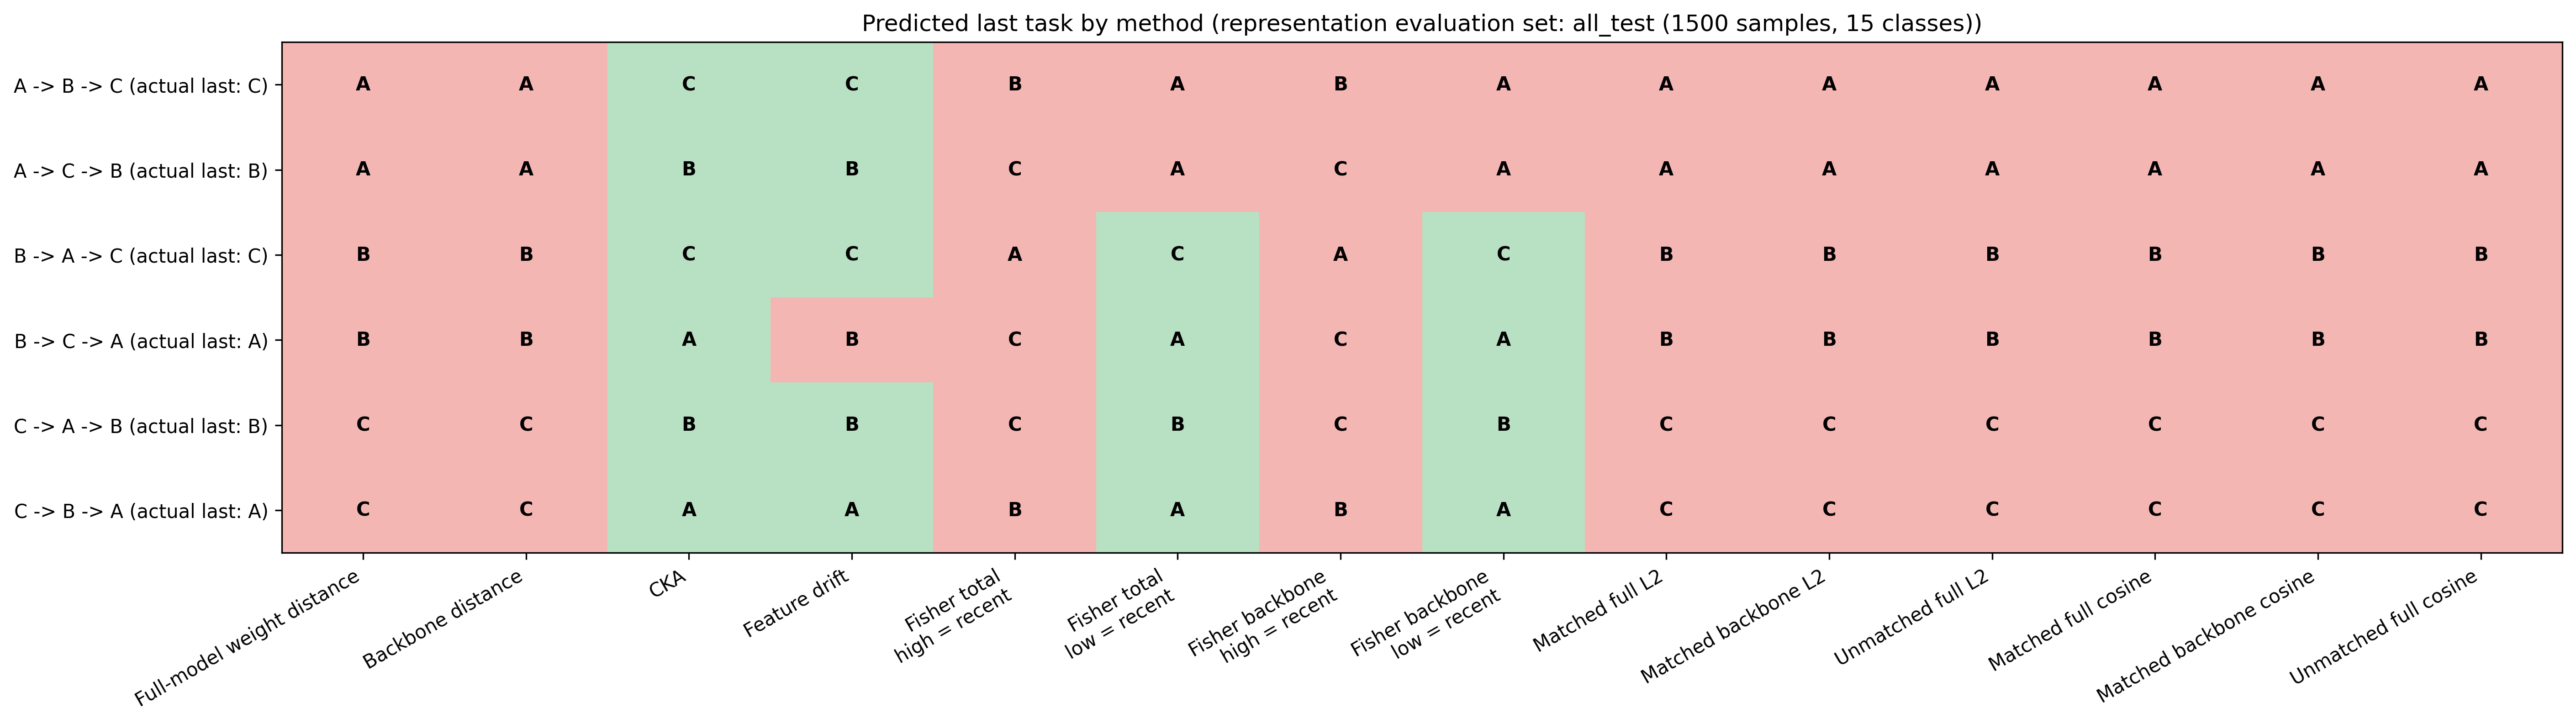
\includegraphics[width=\linewidth]{prediction_matrix.png}
\caption{Predicted last task for every order (rows) and method (columns). Green cells are correct, red cells are wrong. The first two columns and the last six columns, all based on weights, are completely red.}
\label{fig:matrix}
\end{figure}

With only six orders, every single prediction counts for 16.7 percentage points, so the numbers have to be interpreted with care. If a method guessed at random, the chance of getting all six right would be $(1/3)^6 \approx 0.14\%$, of getting at least five right about $1.8\%$, and of getting at least four right about $10\%$. These values assume independent guesses, which is only roughly true here because the six orders share the same three reference models. They still suggest that the CKA result is unlikely to be luck, while the Fisher result with four of six is not distinguishable from chance with this sample size.

\subsubsection{Weight space}

Figure~\ref{fig:weightdist} shows the distances between each final model and the three references. In every order the reference with the smallest distance is the one of the \emph{first} task: the distance to it is roughly 5.5 to 6.2 for the full model, while the distances to the other two references are roughly 7.7 to 8.2. The distances to the references of the second and the last task are close to each other. This is why the lowest-distance rule fails in each order, and why its failures are systematic rather than random. The backbone-only distance shows the same pattern.

\begin{figure}[t]
\centering
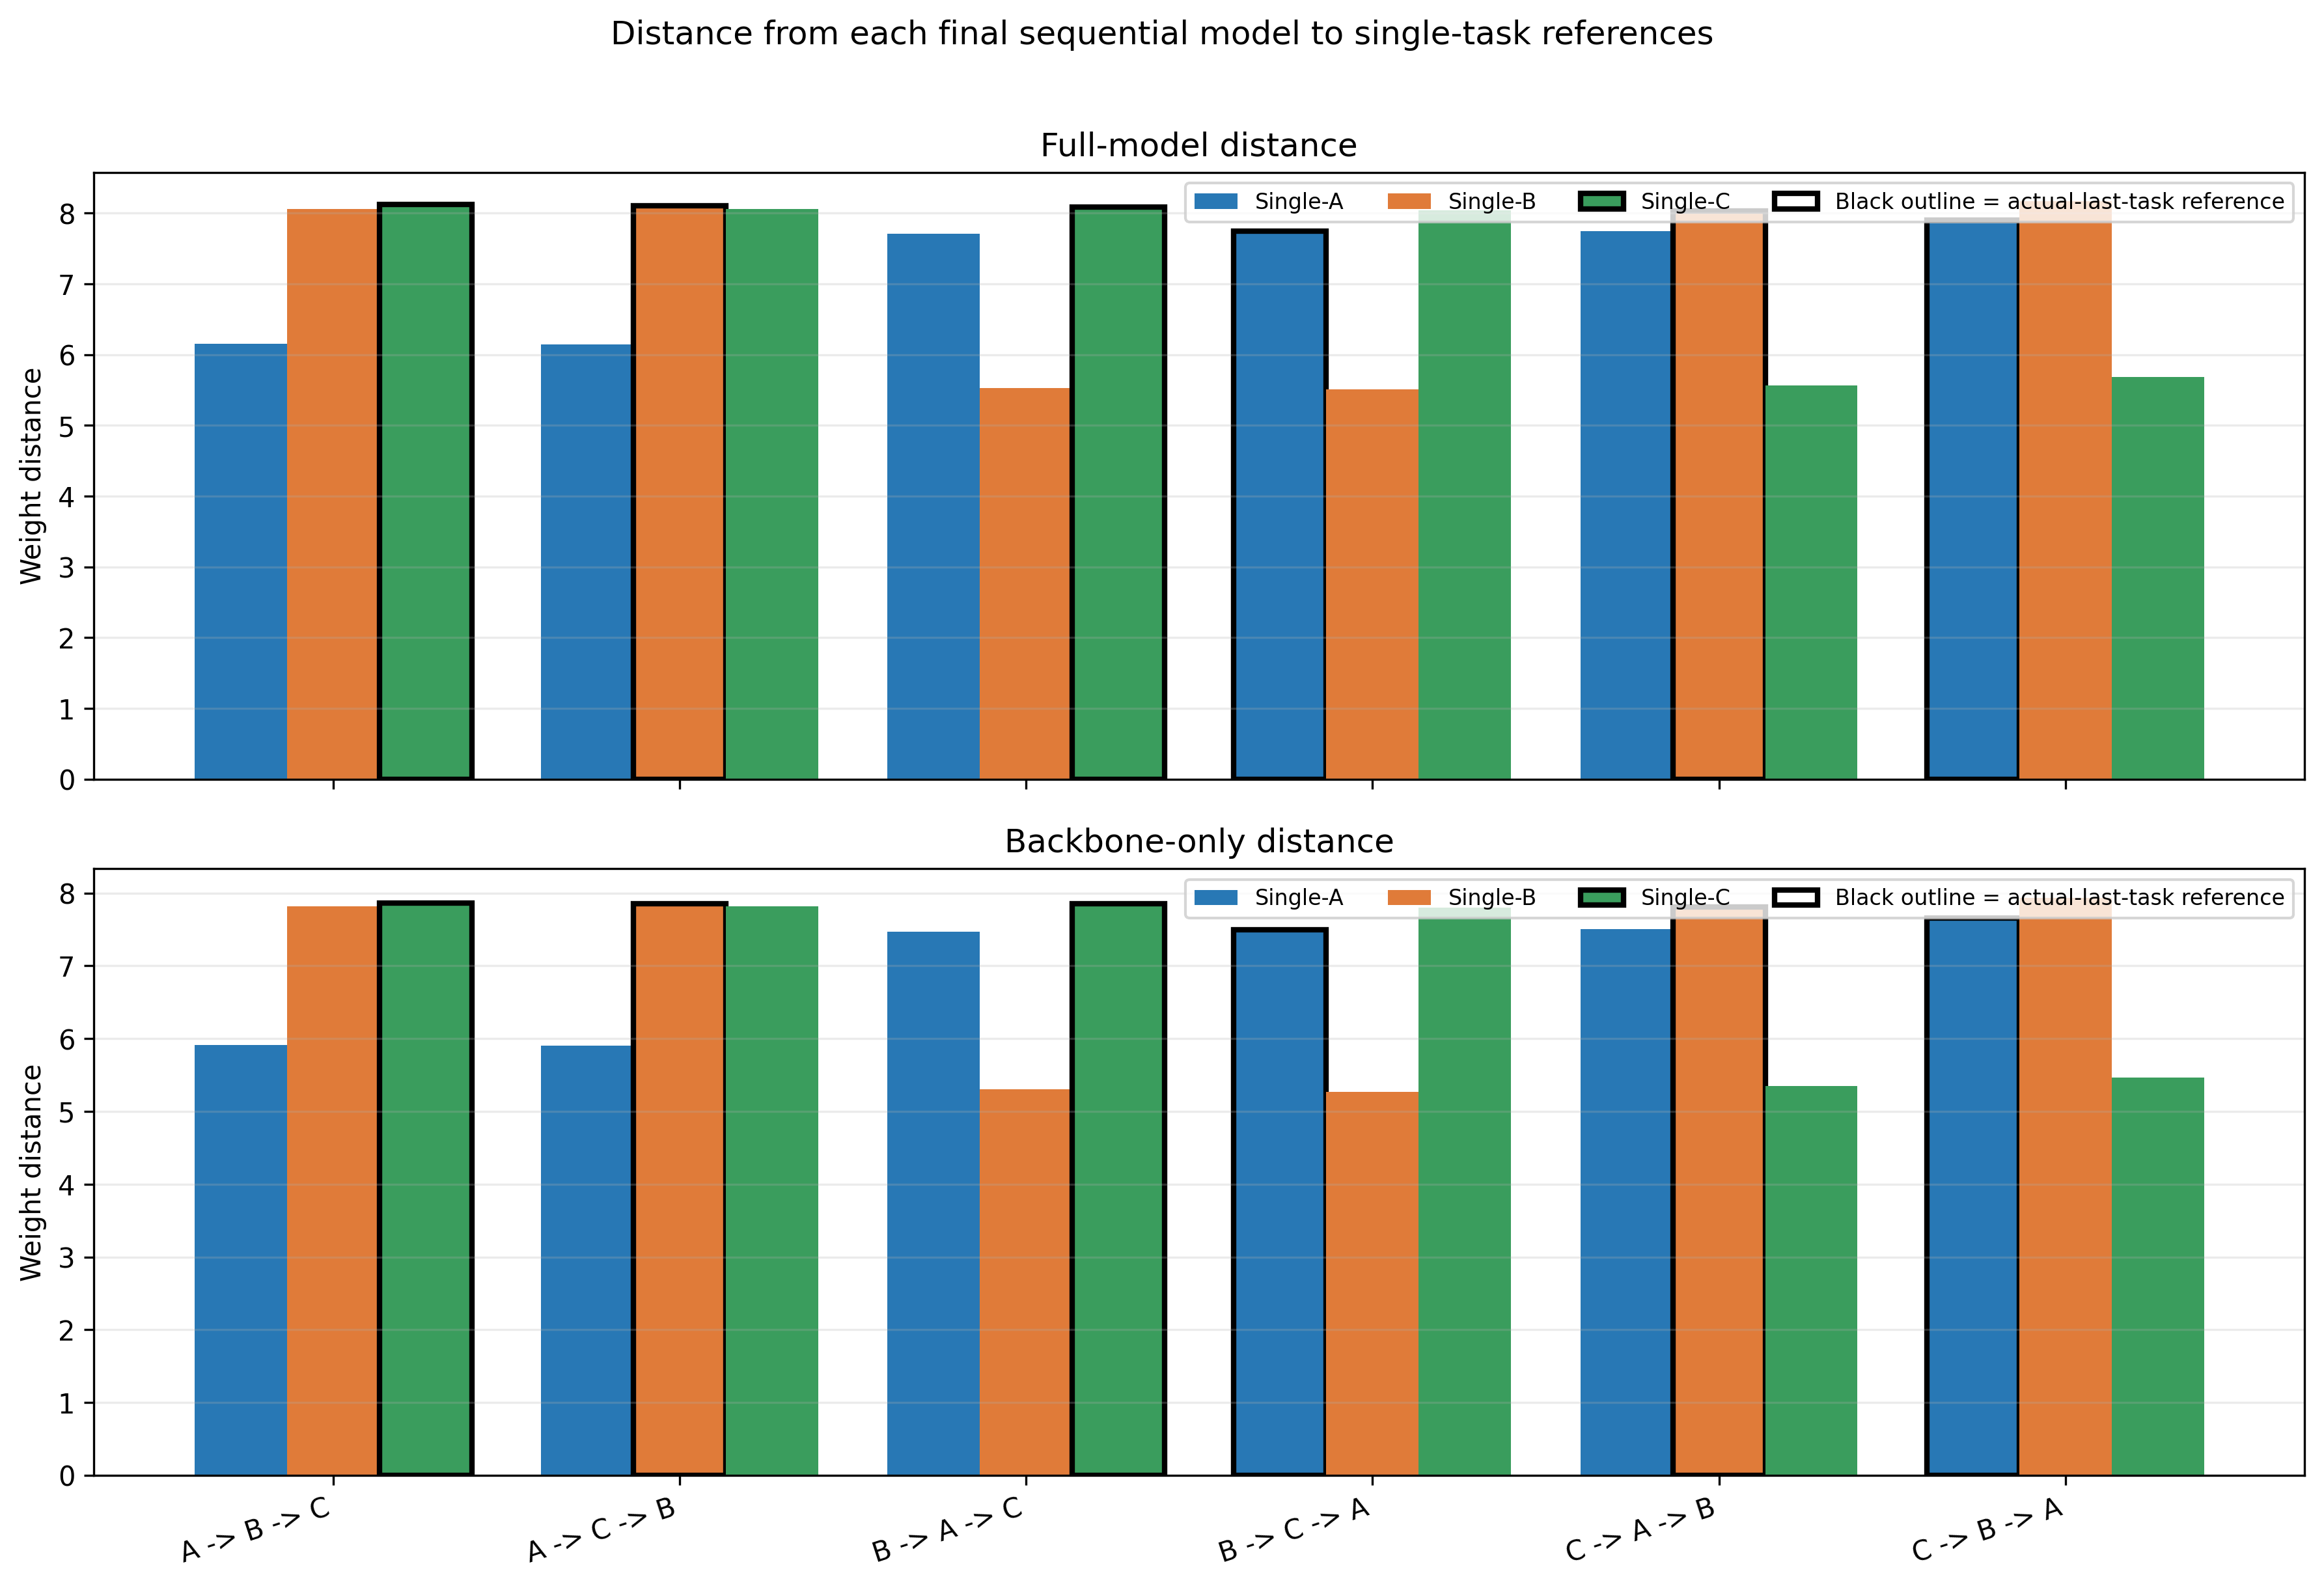
\includegraphics[width=0.88\linewidth]{weight_distance_scores.png}
\caption{L2 distance from each final sequential model to the single-task references (top: all parameters, bottom: backbone only). The black outline marks the reference of the actual last task. The smallest bar belongs to the first task of every order.}
\label{fig:weightdist}
\end{figure}

Weight matching did not change this. Figure~\ref{fig:wm} compares L2 distance and cosine similarity before and after alignment, and in both panels the two markers lie on top of each other for every combination. The analysis found identity permutations, which is the expected outcome when all models are fine-tuned from one shared initialisation. The cosine similarity again separates the first task from the other two (about 0.59 to 0.69 for the first-task reference against about 0.16 to 0.19 for the others), so it points to the wrong task as well. We therefore see no sign that the poor accuracy of the weight distances is caused by neuron ordering. Note, however, that this also means weight matching could not show any benefit in our setup (see Section~\ref{sec:discussion}).

\begin{figure}[t]
\centering
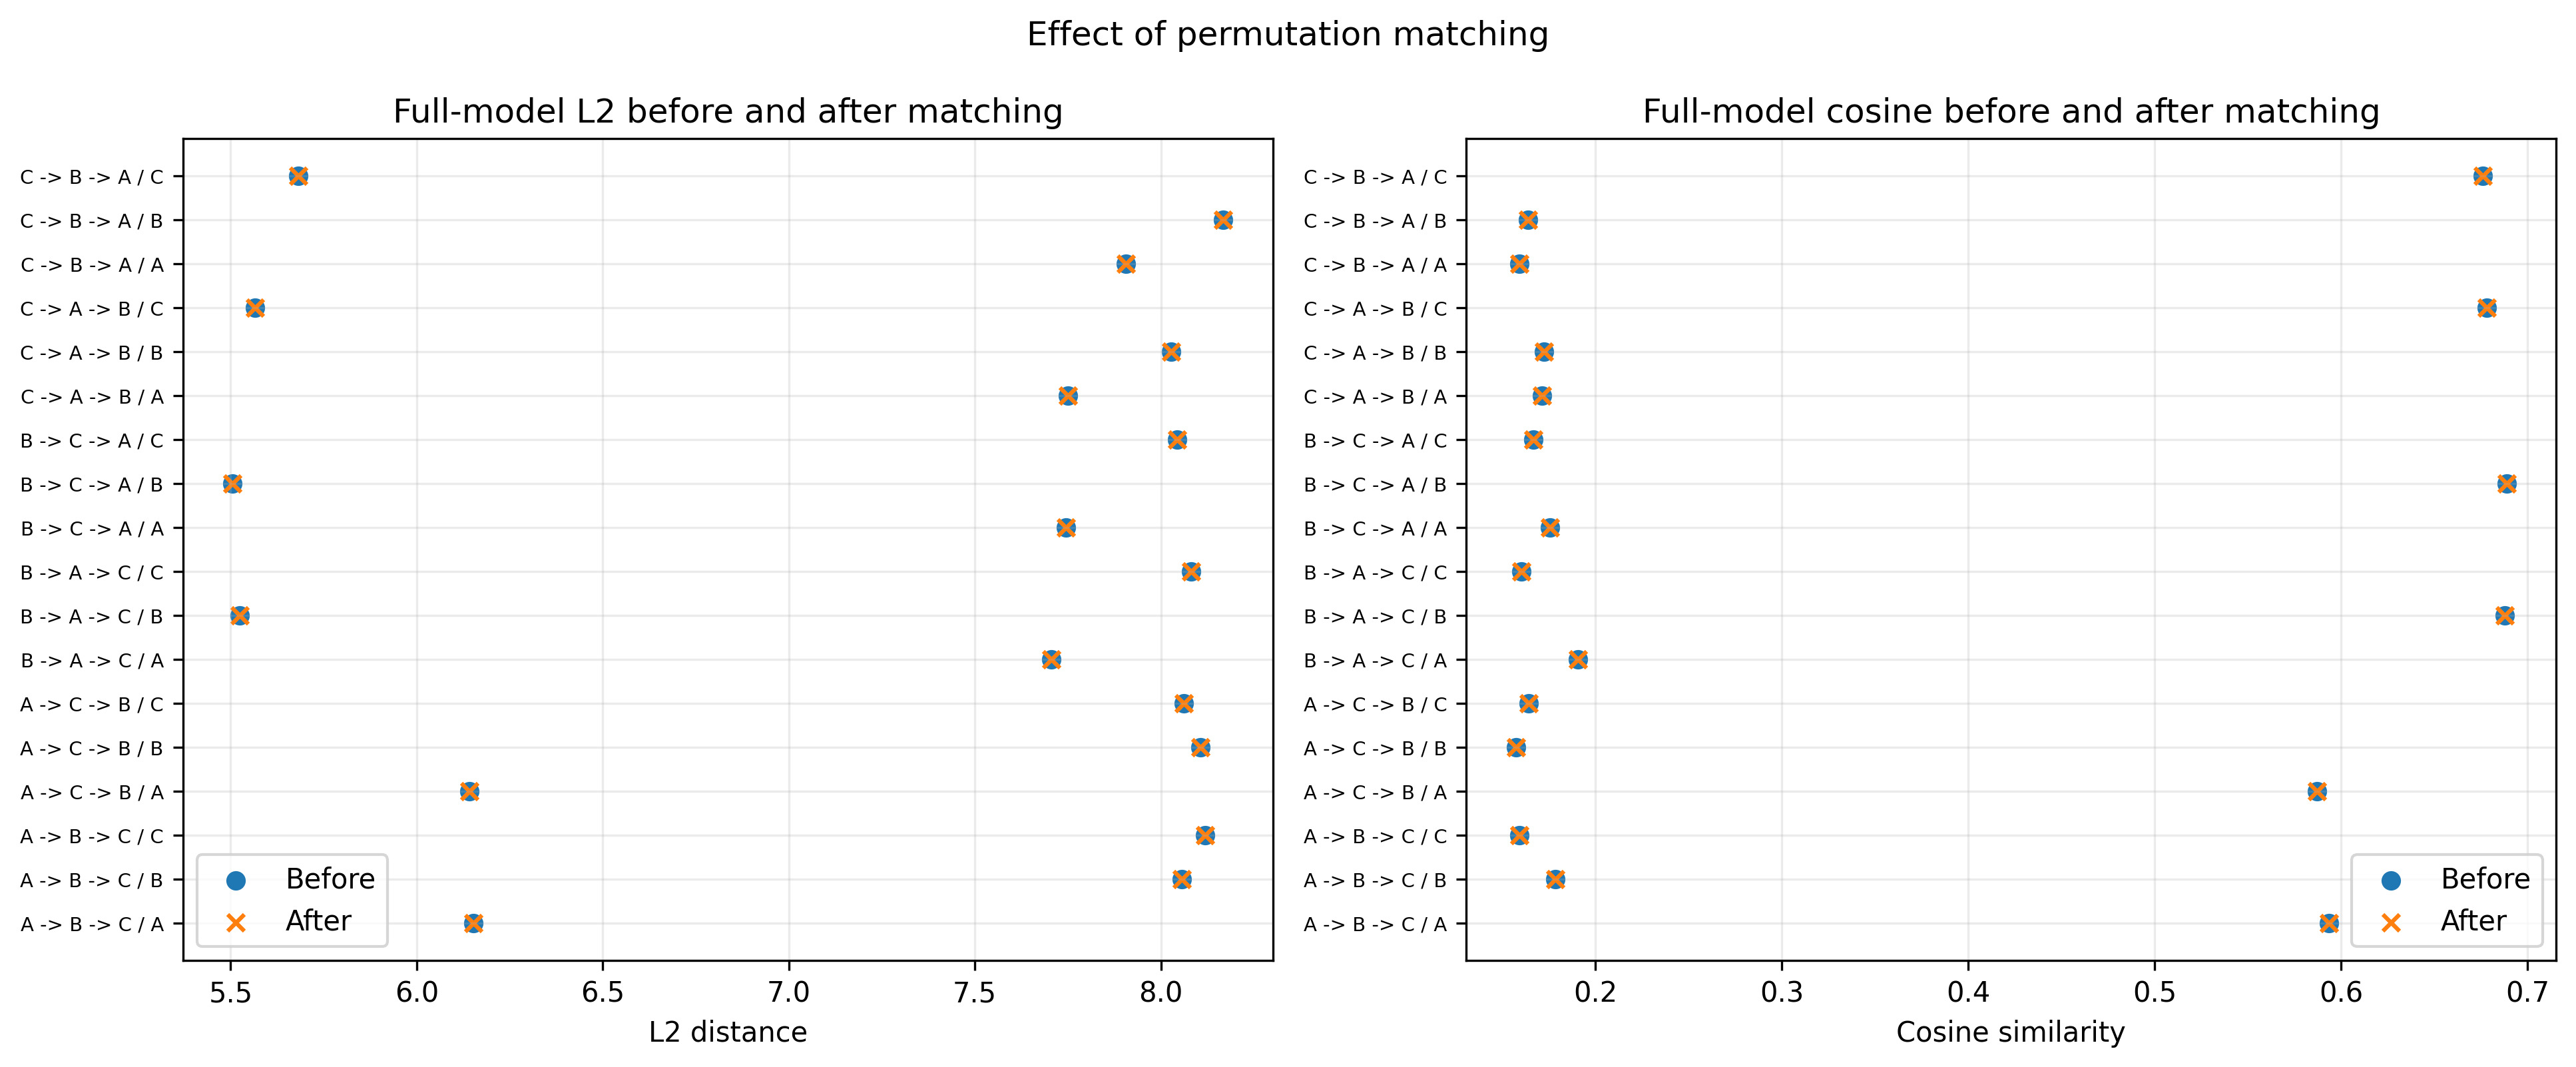
\includegraphics[width=0.95\linewidth]{weight_matching_before_after.png}
\caption{Full-model L2 distance (left) and cosine similarity (right) before and after weight matching. Each row is one order and one reference; the markers coincide.}
\label{fig:wm}
\end{figure}

\subsubsection{Representation space}

In representation space the picture is different. Figure~\ref{fig:cka} shows that in all six orders the highest CKA belongs to the reference of the actual last task. The values for the last-task reference lie between 0.63 and 0.75, while the other references reach at most 0.43. The gap is large and does not depend on which of the three tasks is last.

\begin{figure}[t]
\centering
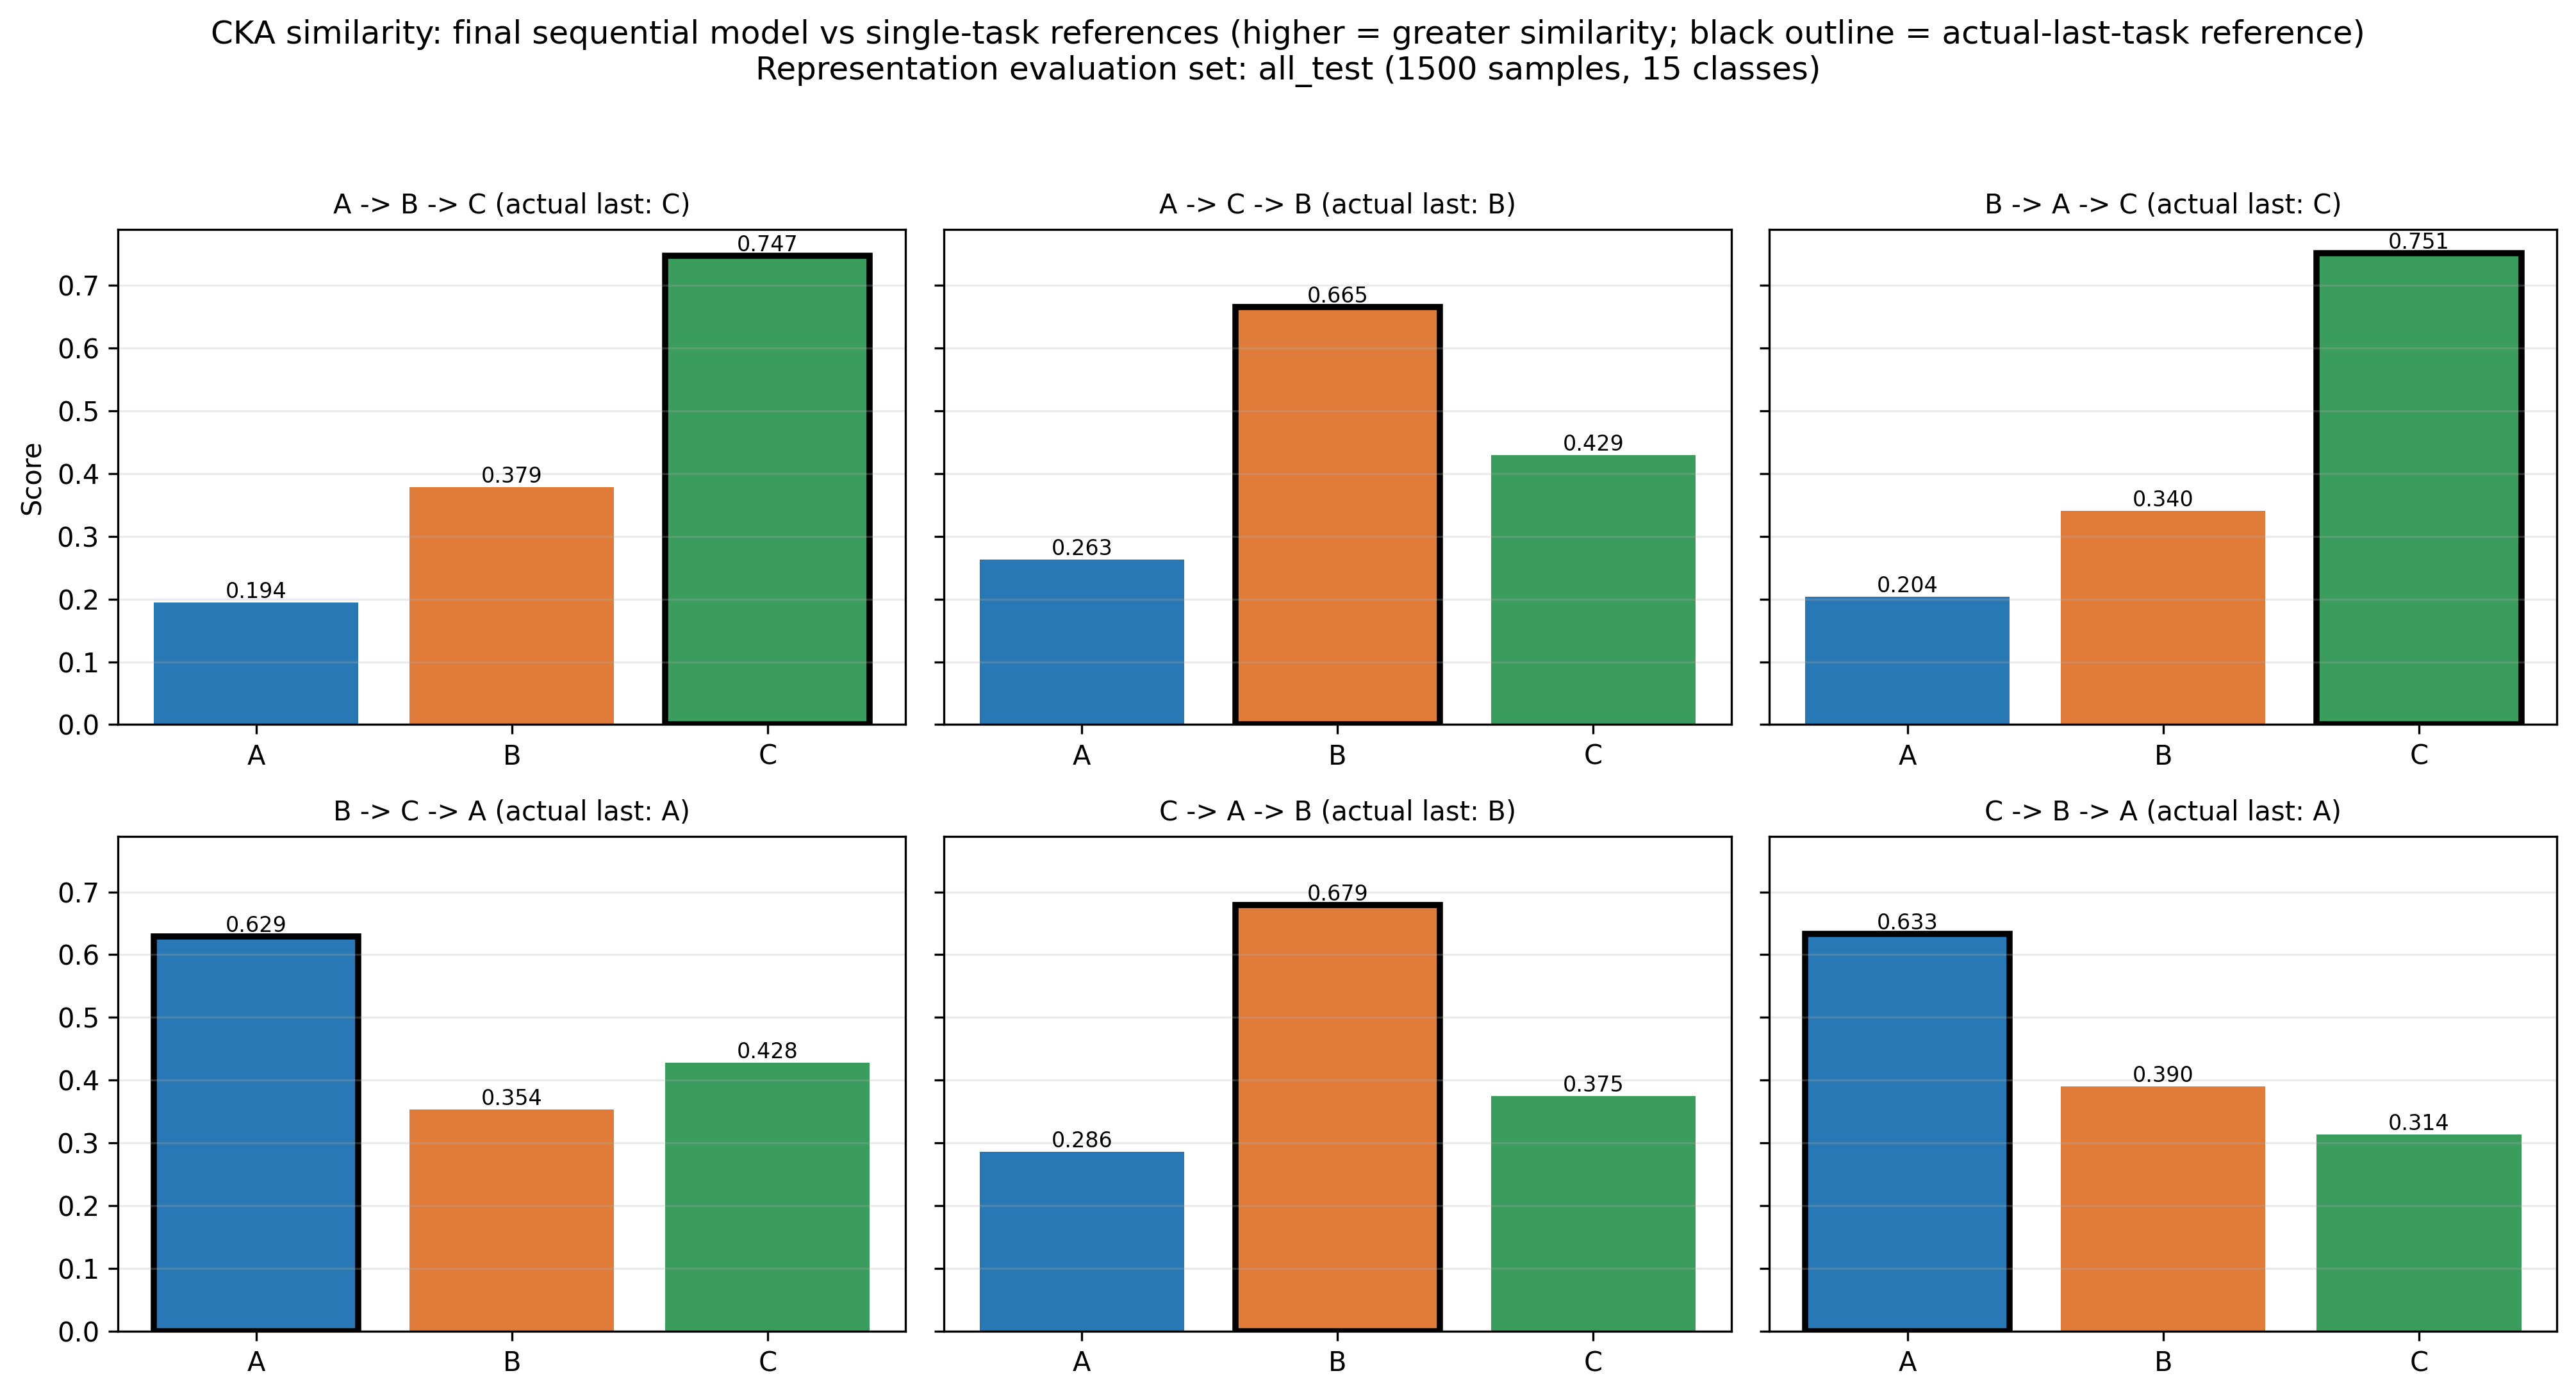
\includegraphics[width=0.88\linewidth]{cka_similarity.png}
\caption{Linear CKA between each final sequential model and the single-task references on the 1500 test images. The black outline marks the reference of the actual last task.}
\label{fig:cka}
\end{figure}

Feature drift (Figure~\ref{fig:drift}) points the same way, but the margins are much smaller. The values are all between about 0.54 and 0.62, and the differences between the lowest and the second-lowest drift are between about 0.006 and 0.04. The single failure is the order \order{B}{C}{A}, where the drift is lowest for \task{B} (0.571) and slightly higher for \task{A} (0.579), the actual last task. So the signal exists, but it is weaker and more fragile than the one in CKA.

\begin{figure}[t]
\centering
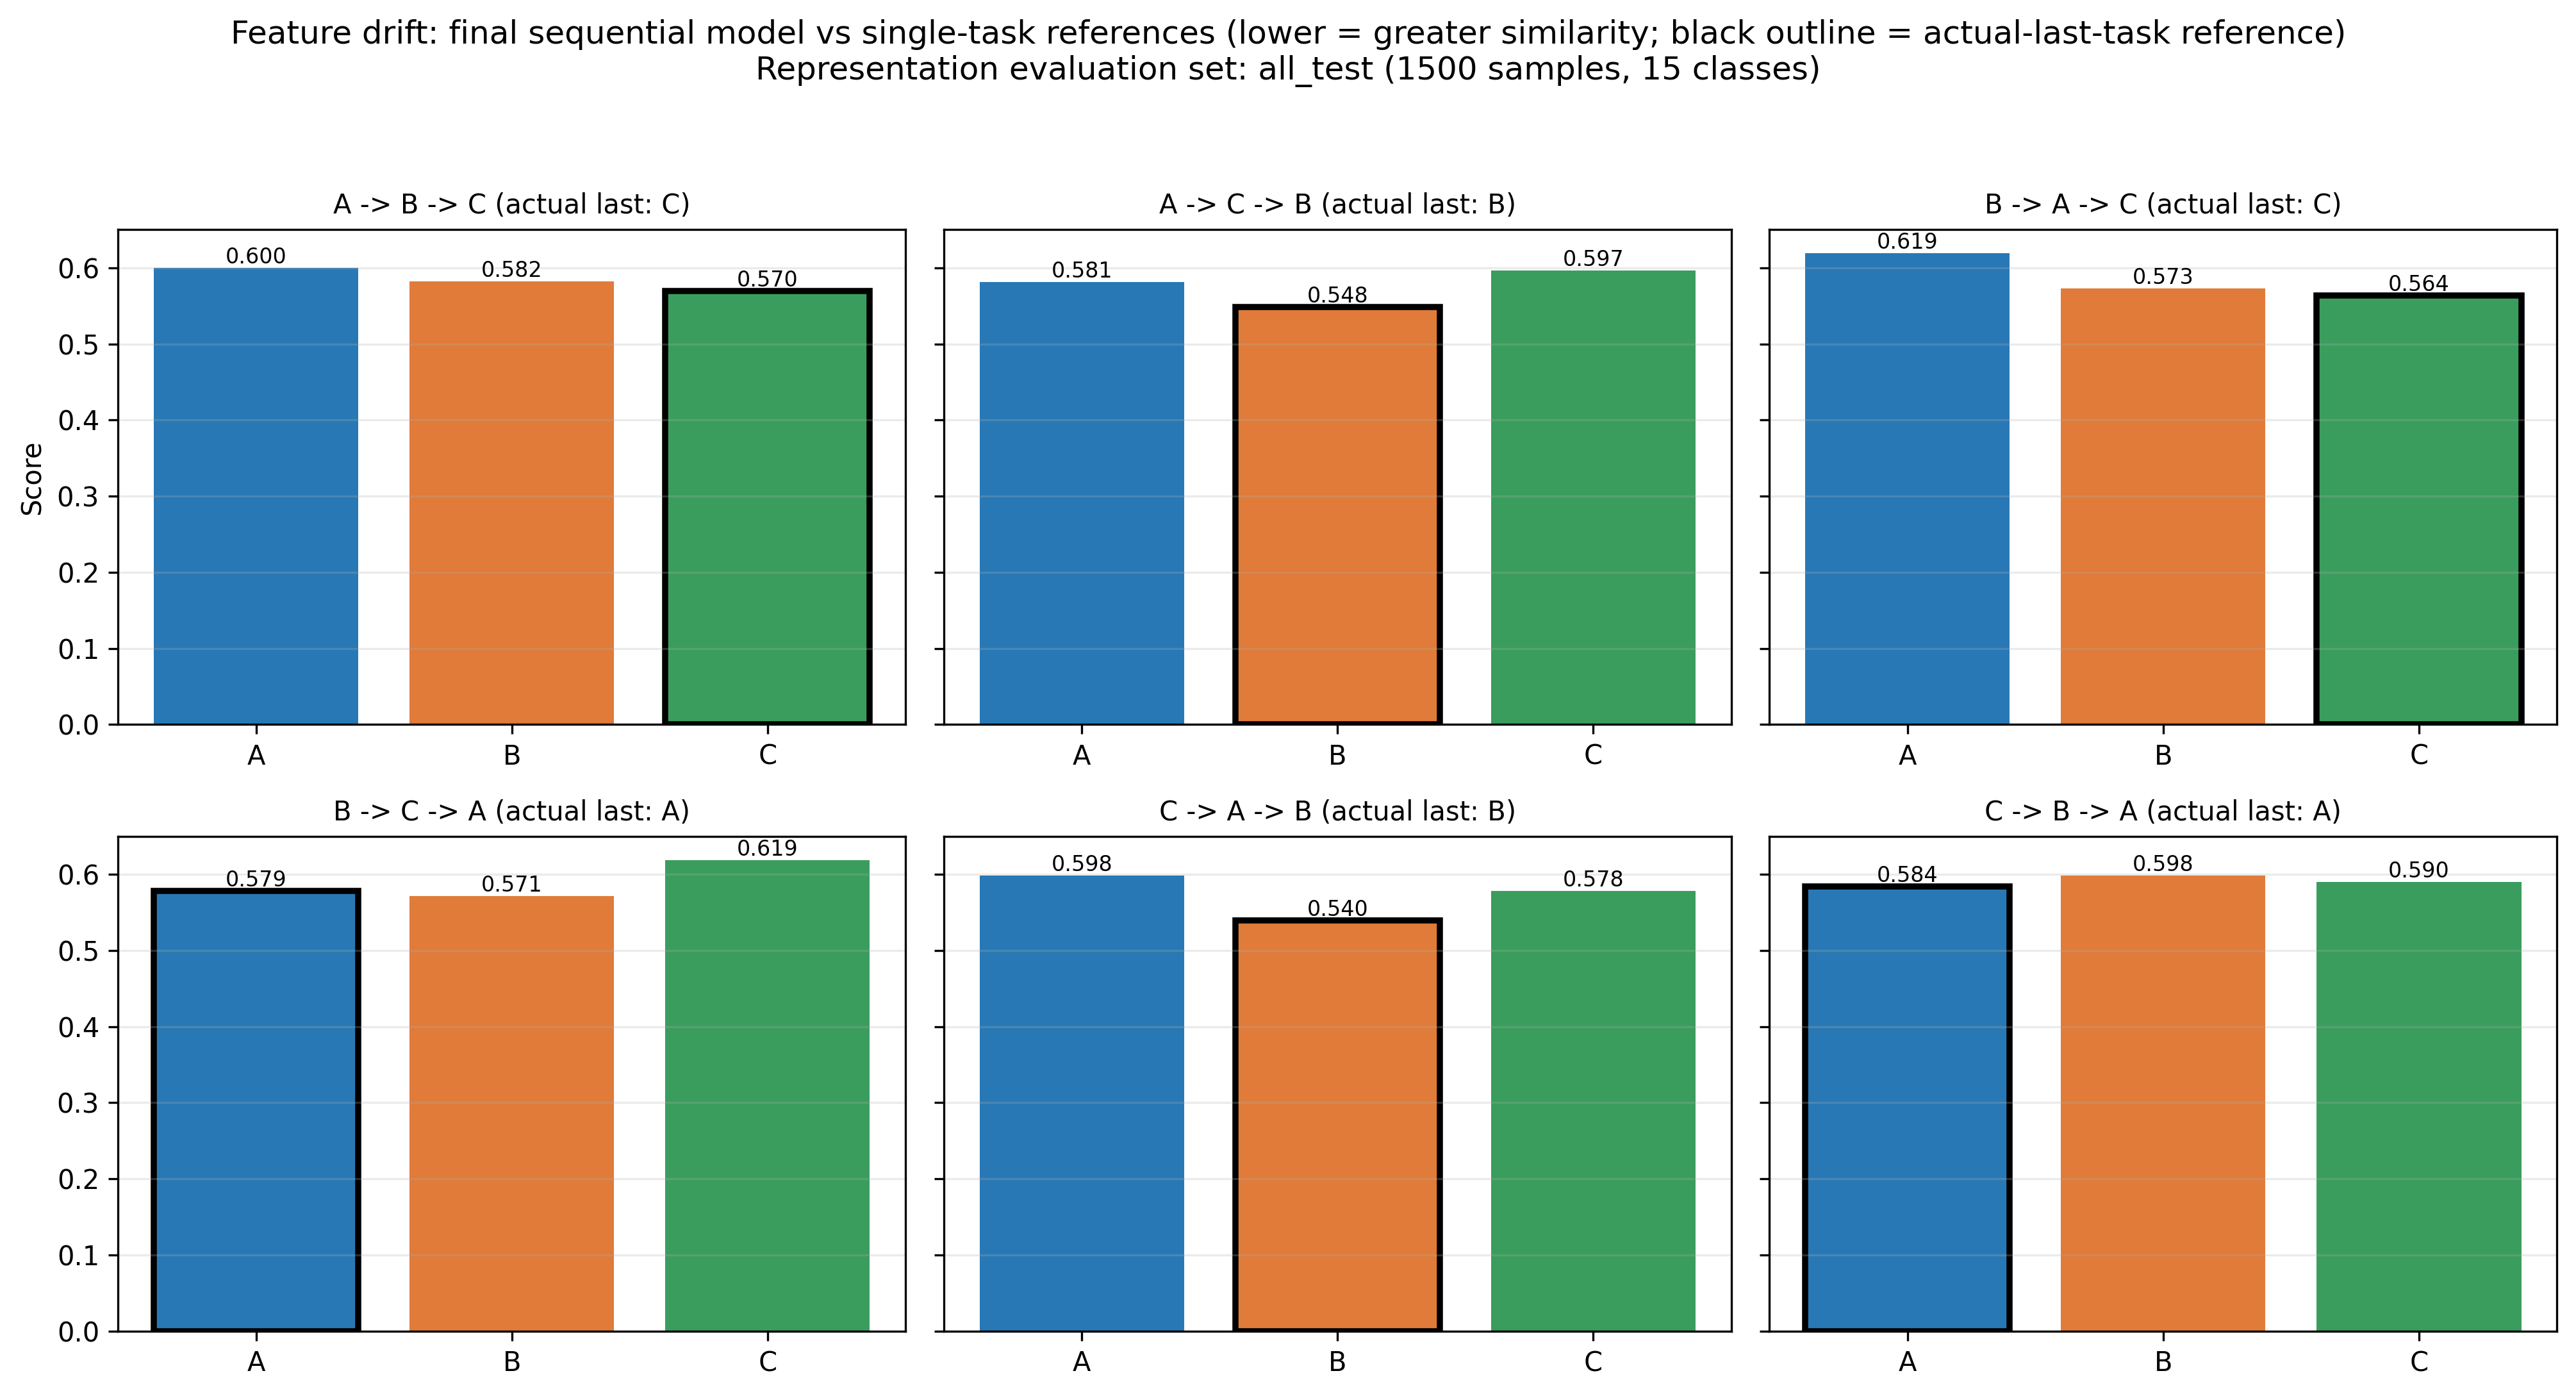
\includegraphics[width=0.88\linewidth]{feature_drift.png}
\caption{Feature drift between each final sequential model and the single-task references on the same 1500 images (lower means more similar). The black outline marks the reference of the actual last task.}
\label{fig:drift}
\end{figure}

\subsubsection{Fisher information}

Figure~\ref{fig:fisher} shows the Fisher traces. They range from about 5{,}000 to 12{,}000, and the backbone trace is only slightly below the total trace, so the heads contribute little. Under ``low is recent'' the last task has the smallest trace in four of the six orders (\order{B}{A}{C}, \order{B}{C}{A}, \order{C}{A}{B} and \order{C}{B}{A}). In the two orders that start with \task{A}, the smallest trace is that of \task{A} itself. In \order{C}{A}{B} the three traces are very close (roughly 7{,}600 to 8{,}000), so the correct answer there rests on a small difference. Used to guess the complete order, the Fisher ranking was correct in only one of six cases, which is close to the chance level of $1/6$.

\begin{figure}[t]
\centering
\begin{subfigure}[t]{0.58\linewidth}
  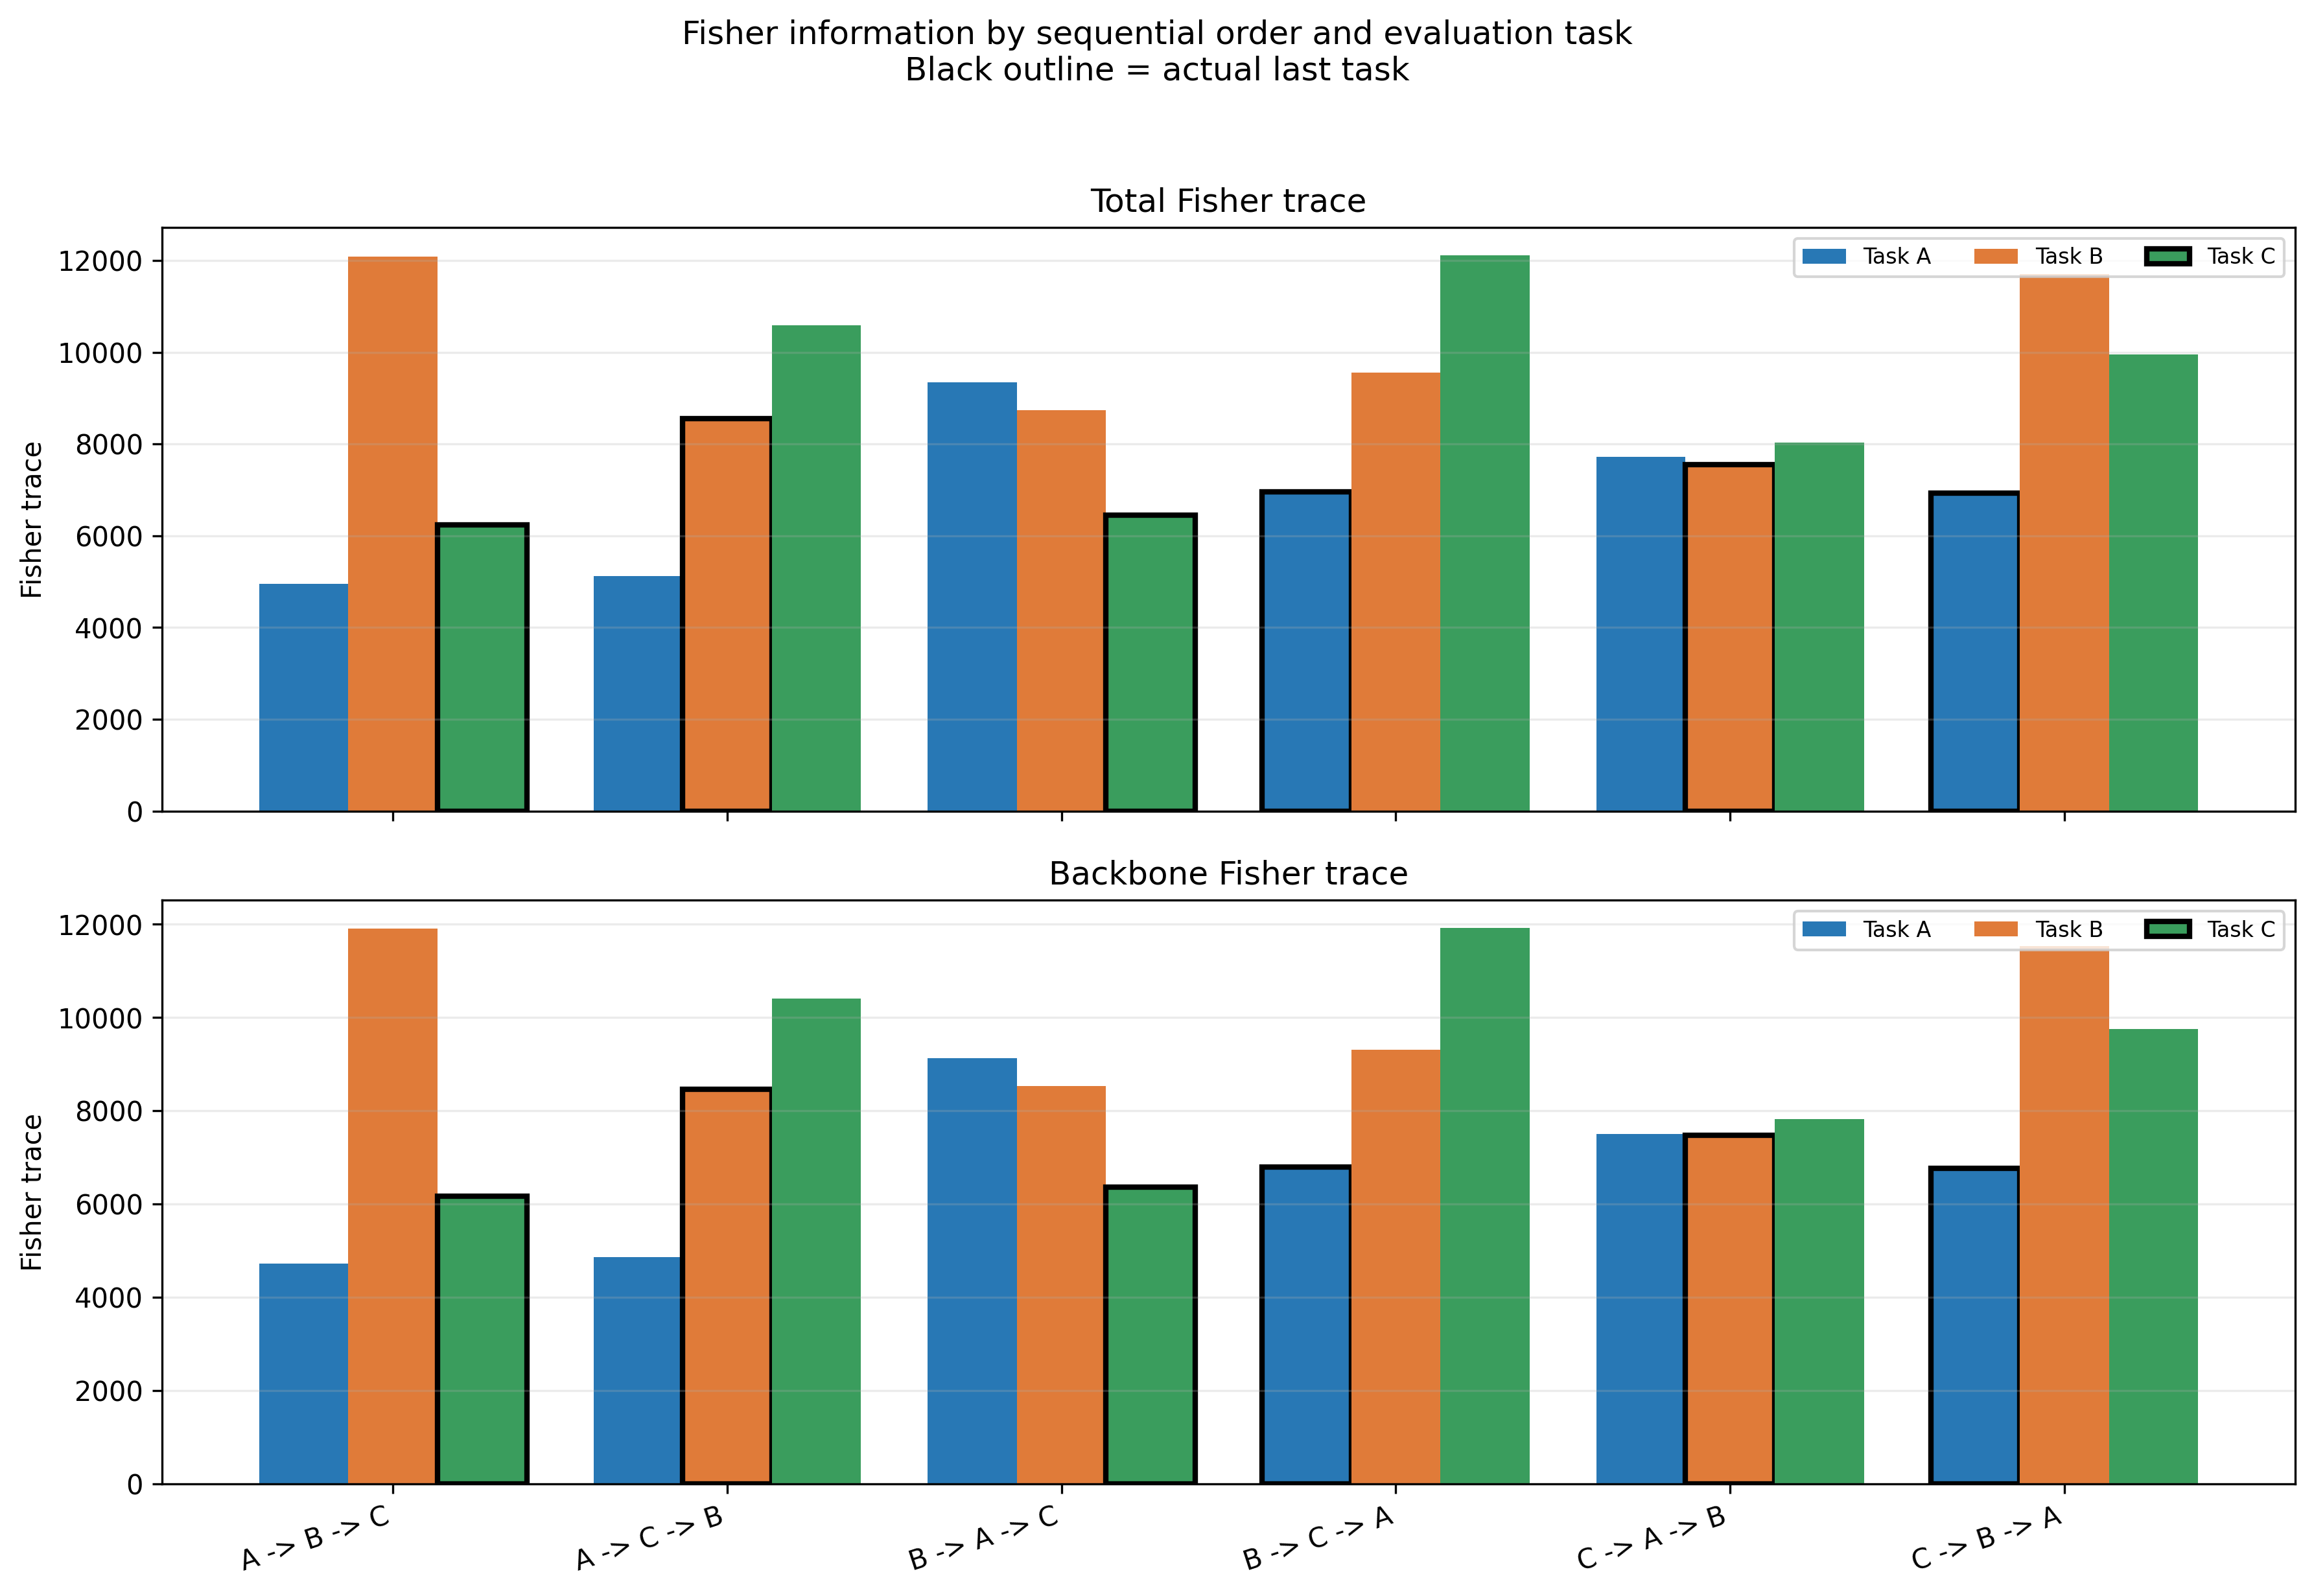
\includegraphics[width=\linewidth]{fisher_information_scores.png}
  \caption{Fisher trace per order and evaluation task.}
\end{subfigure}\hfill
\begin{subfigure}[t]{0.40\linewidth}
  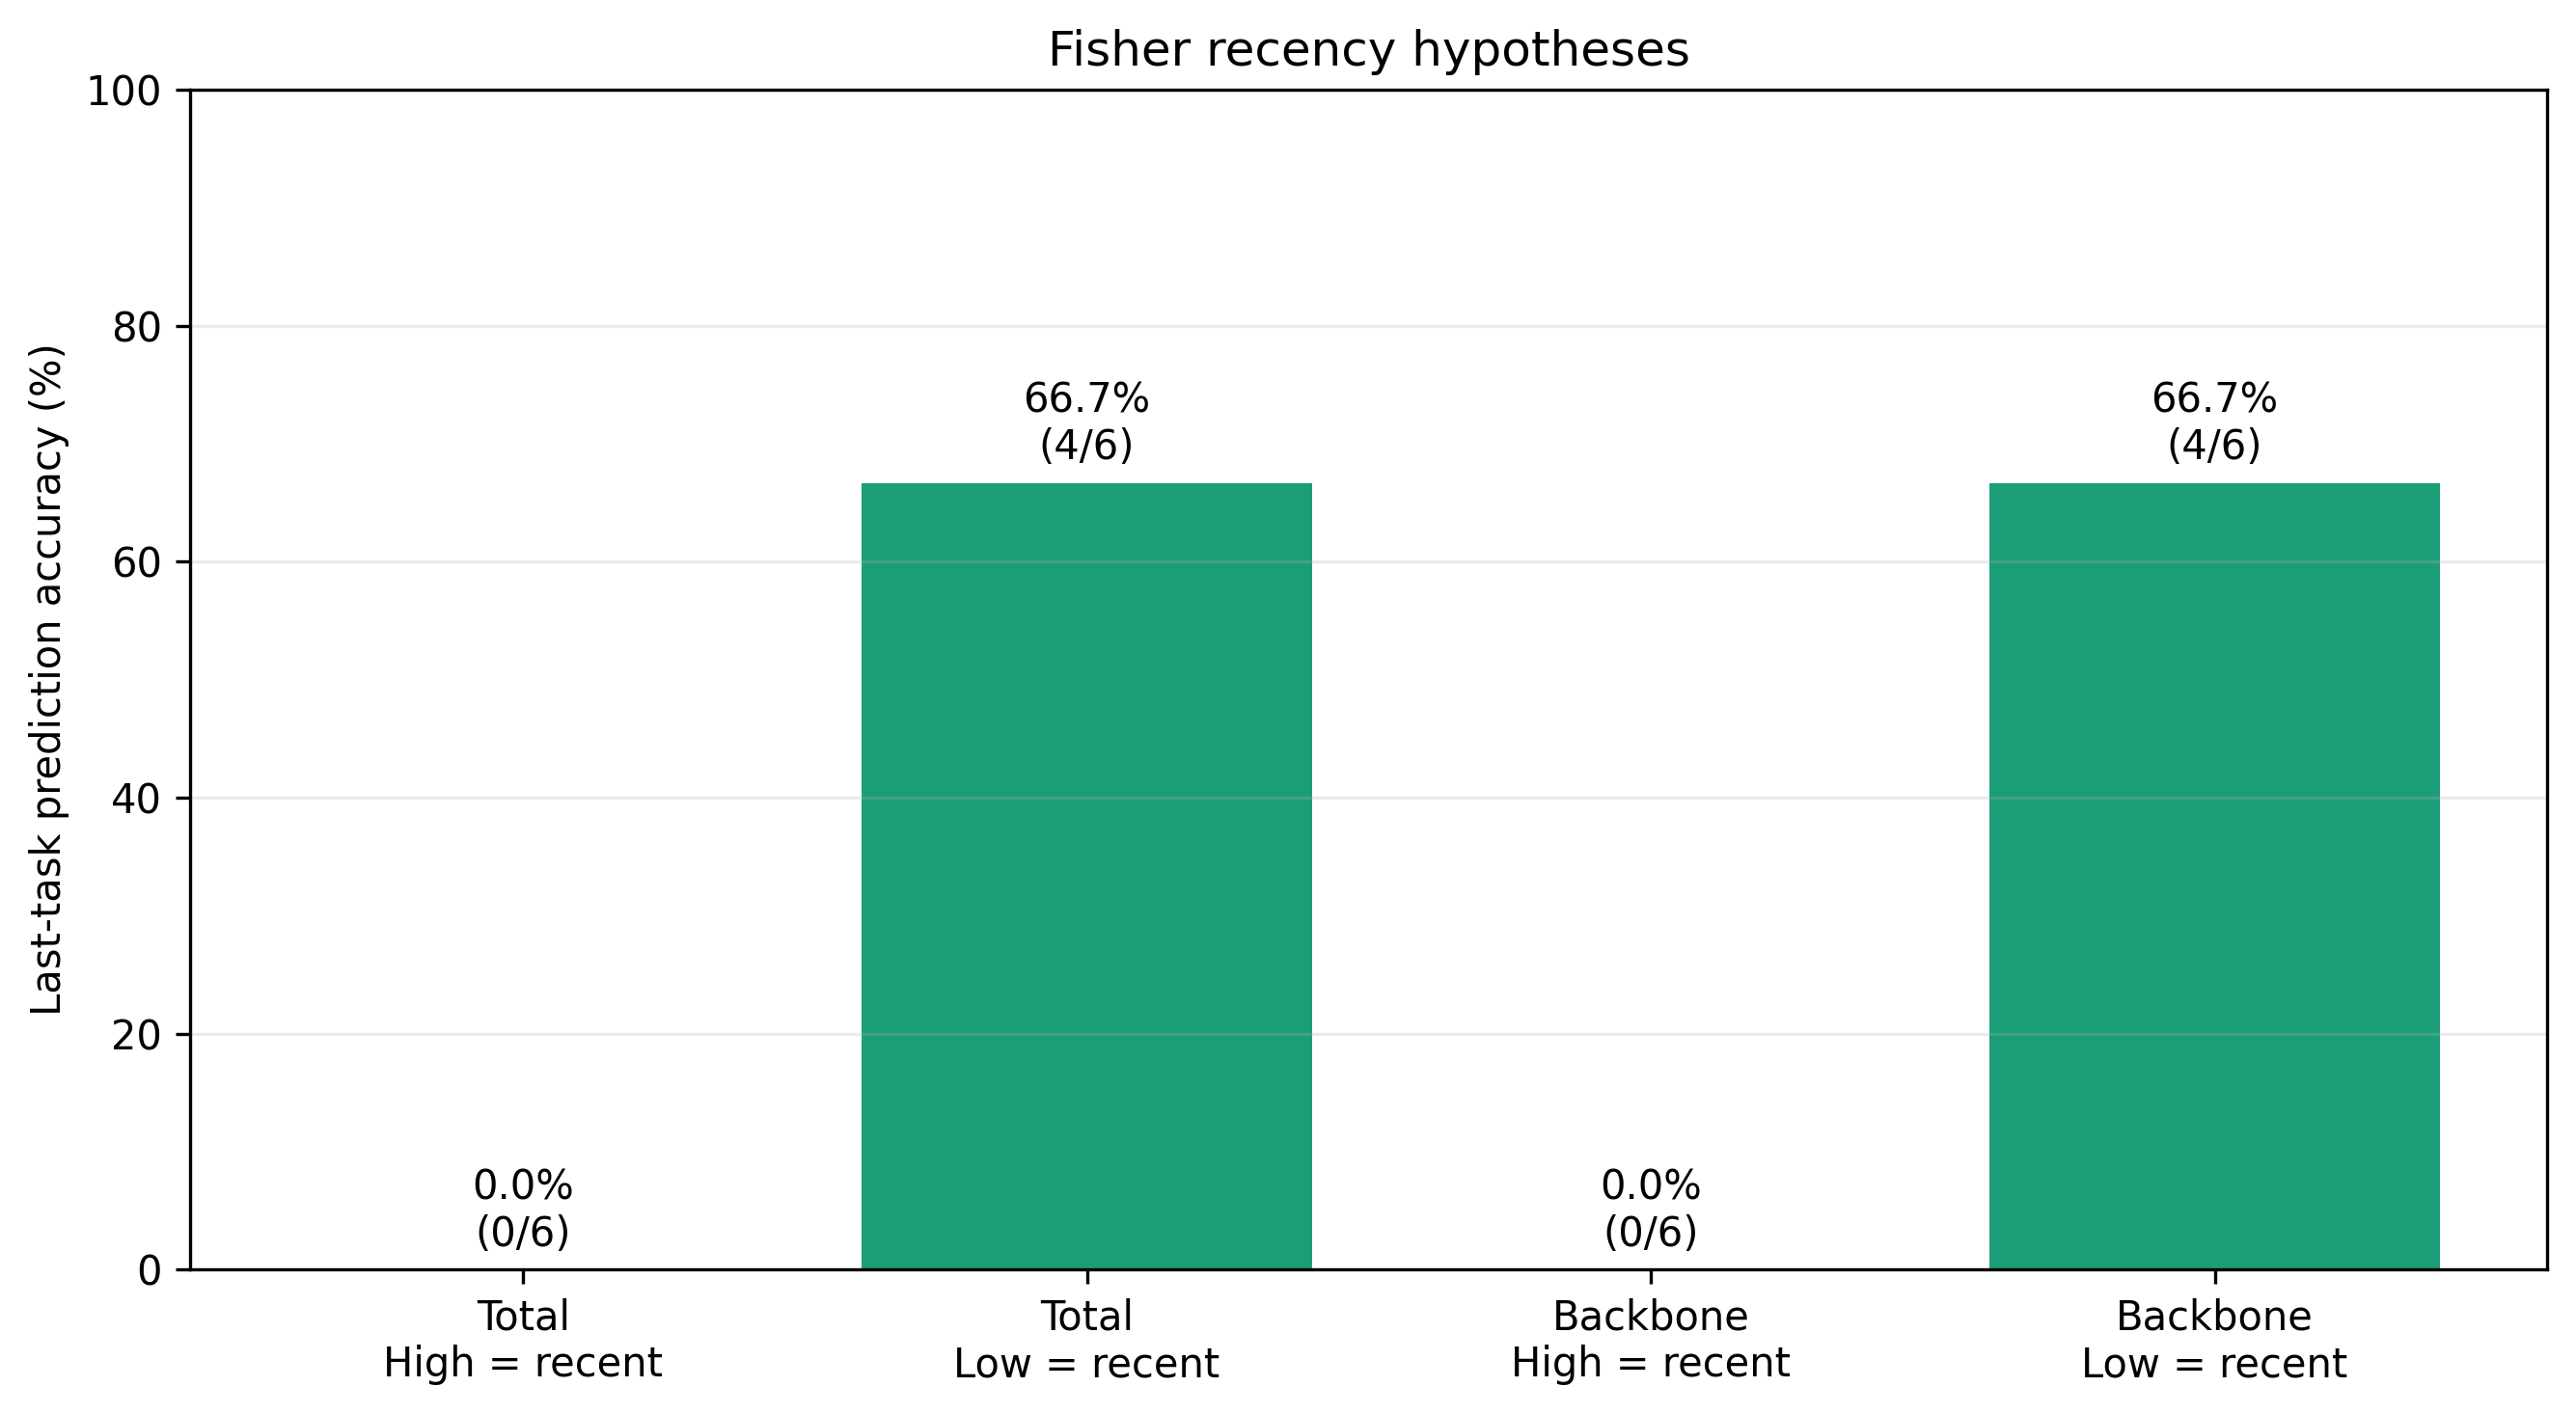
\includegraphics[width=\linewidth]{fisher_hypothesis_accuracy.png}
  \caption{Last-task accuracy of the two readings.}
\end{subfigure}
\caption{Fisher information of the final sequential models. In (a), the black outline marks the actual last task.}
\label{fig:fisher}
\end{figure}

\subsection{RQ2: Predicting the full order}

None of the methods gives the complete order directly. The Fisher ranking is the only one that produces a full order by itself, and it reached 1/6. However, two of our results complement each other. Weight distance, which fails at the last task, picked the first task in all six orders (Figure~\ref{fig:matrix} and Figure~\ref{fig:weightdist}). CKA picks the last task in all six orders. With three tasks, knowing the first and the last task leaves only one possibility for the middle one. Table~\ref{tab:order} shows the result: all six orders are reconstructed correctly.

\begin{table}[t]
\centering
\caption{Order reconstruction from the first task (lowest weight distance) and the last task (highest CKA). The middle task is the remaining one.}
\label{tab:order}
\begin{tabular}{lccc}
\toprule
True order & First (weight distance) & Last (CKA) & Reconstructed order \\
\midrule
\order{A}{B}{C} & \task{A} & \task{C} & \order{A}{B}{C} \\
\order{A}{C}{B} & \task{A} & \task{B} & \order{A}{C}{B} \\
\order{B}{A}{C} & \task{B} & \task{C} & \order{B}{A}{C} \\
\order{B}{C}{A} & \task{B} & \task{A} & \order{B}{C}{A} \\
\order{C}{A}{B} & \task{C} & \task{B} & \order{C}{A}{B} \\
\order{C}{B}{A} & \task{C} & \task{A} & \order{C}{B}{A} \\
\bottomrule
\end{tabular}
\end{table}

We want to be clear about the limits of this result. The rule ``weight distance finds the first task'' was noticed after looking at the results, it was not a hypothesis we set up beforehand. It also only works because three tasks are few: the middle one is determined by elimination. With four or more tasks, the positions between the first and the last would remain open, and we have no method that ranks those. So we view this as an observation for this small setting, not as a general way of recovering a training history.

\subsection{RQ3: Forgetting}

Figure~\ref{fig:forgetting} shows the forgetting of each task in each order. The bar of the last task is always zero, which is true by definition, since there is no later stage. The tasks that were learned earlier show clear losses. Reading the values off the plot, the forgetting of earlier tasks lies between roughly 0.23 and 0.45 accuracy points, on tasks where chance accuracy is 0.2, so a large part of what was learned is lost. In all six orders the first task shows more forgetting than the second task, although the difference is small in some cases (for example \order{A}{C}{B}, where both are about 0.3). The largest value appears for \task{C} in \order{C}{B}{A}. As the heads of earlier tasks are frozen, the loss must come from the change of the shared backbone.

\begin{figure}[t]
\centering
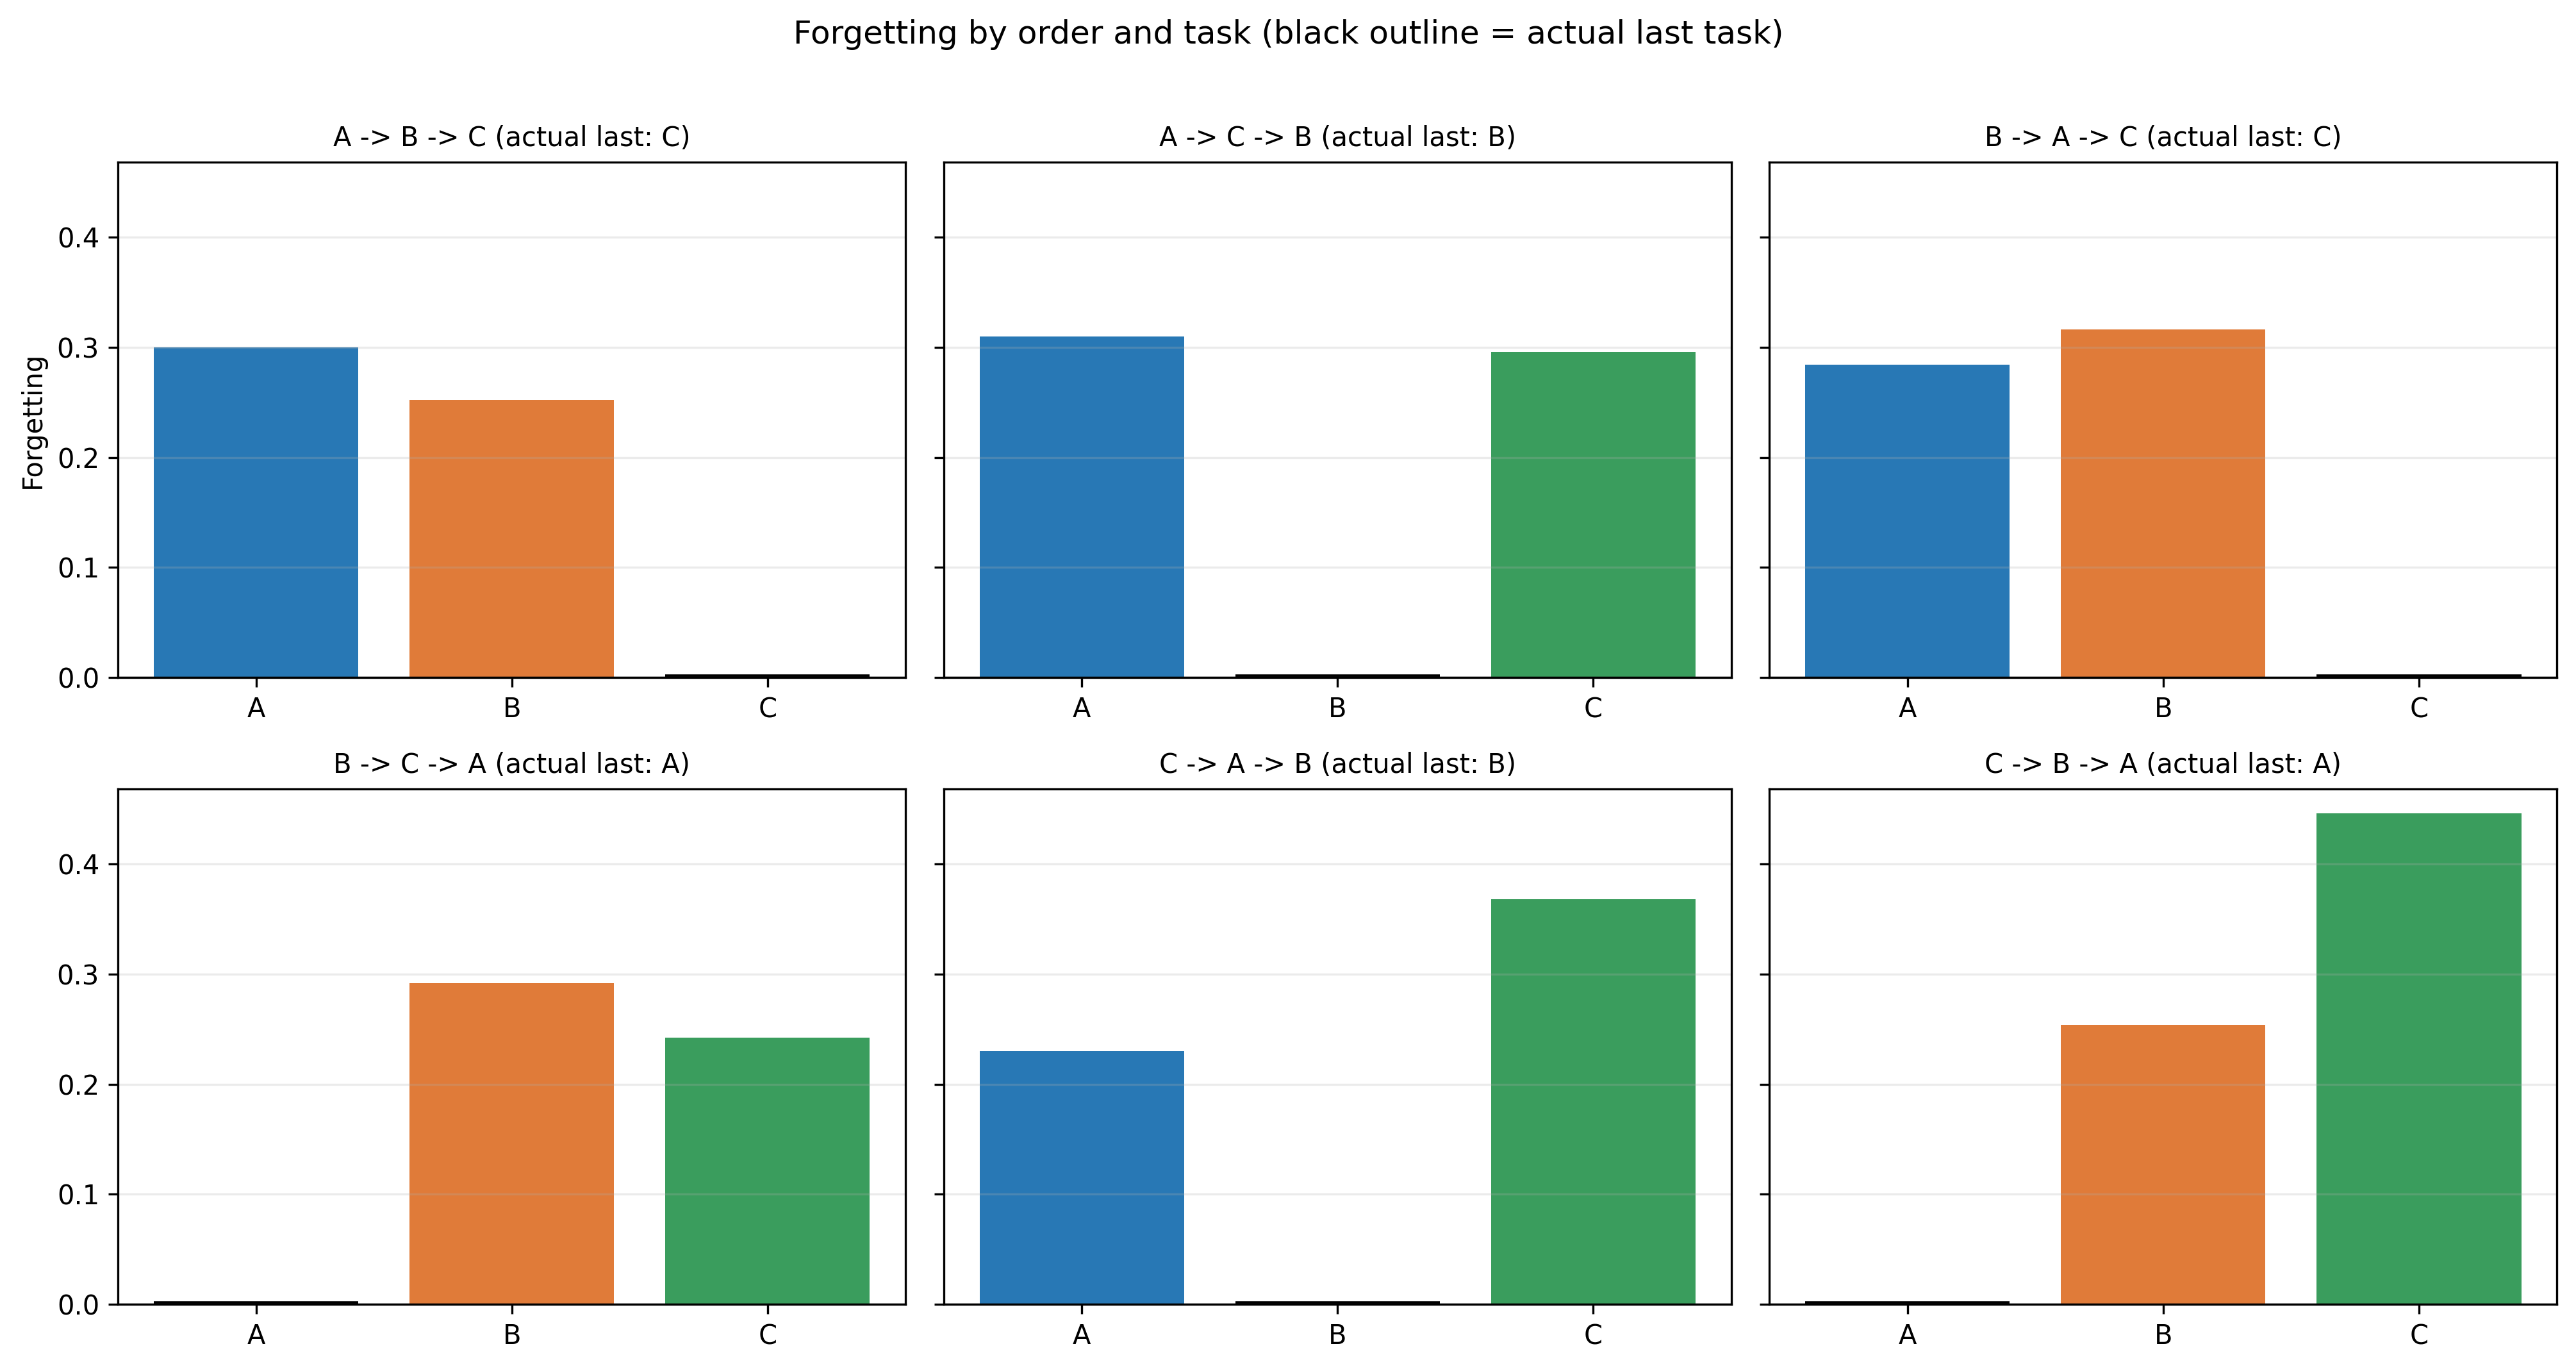
\includegraphics[width=0.88\linewidth]{forgetting_by_order.png}
\caption{Forgetting per task and order (accuracy right after learning the task minus final accuracy). The last task has zero forgetting by definition.}
\label{fig:forgetting}
\end{figure}

An important caveat is the training length. All stages ran for 20 epochs, and the amount of forgetting can depend on how long each task is trained. With more epochs the numbers could look different, in either direction, and we did not test this.

\subsection{Additional diagnostics}

Loss barriers and Jacobian sensitivity were computed as supporting diagnostics. We did not define a prediction rule for them and do not count them as results for RQ1.

For the loss barrier (Figure~\ref{fig:diag}a), the largest barrier height belongs to the reference of the actual last task in all six orders, and the barrier area is largest for it in five of six (the exception is \order{C}{B}{A}, where \textsf{Single-B} has the largest area). We did not investigate the reason. In particular, the loss curves show a high loss at $\alpha=0$ for some references on the task they were trained for, which we have not explained, so we do not want to draw conclusions from these plots.

For Jacobian sensitivity (Figure~\ref{fig:diag}b), the final model is most sensitive on the last task in most orders, but not in all of them: in \order{B}{C}{A} the sensitivity on \task{C} is higher than on the actual last task \task{A}. The three colour channels contribute almost equally, with channel values between about 0.010 and 0.035 and no channel dominating. Since higher sensitivity does not imply that a task was learned recently, we only treat these plots as background.

\begin{figure}[t]
\centering
\begin{subfigure}[t]{0.48\linewidth}
  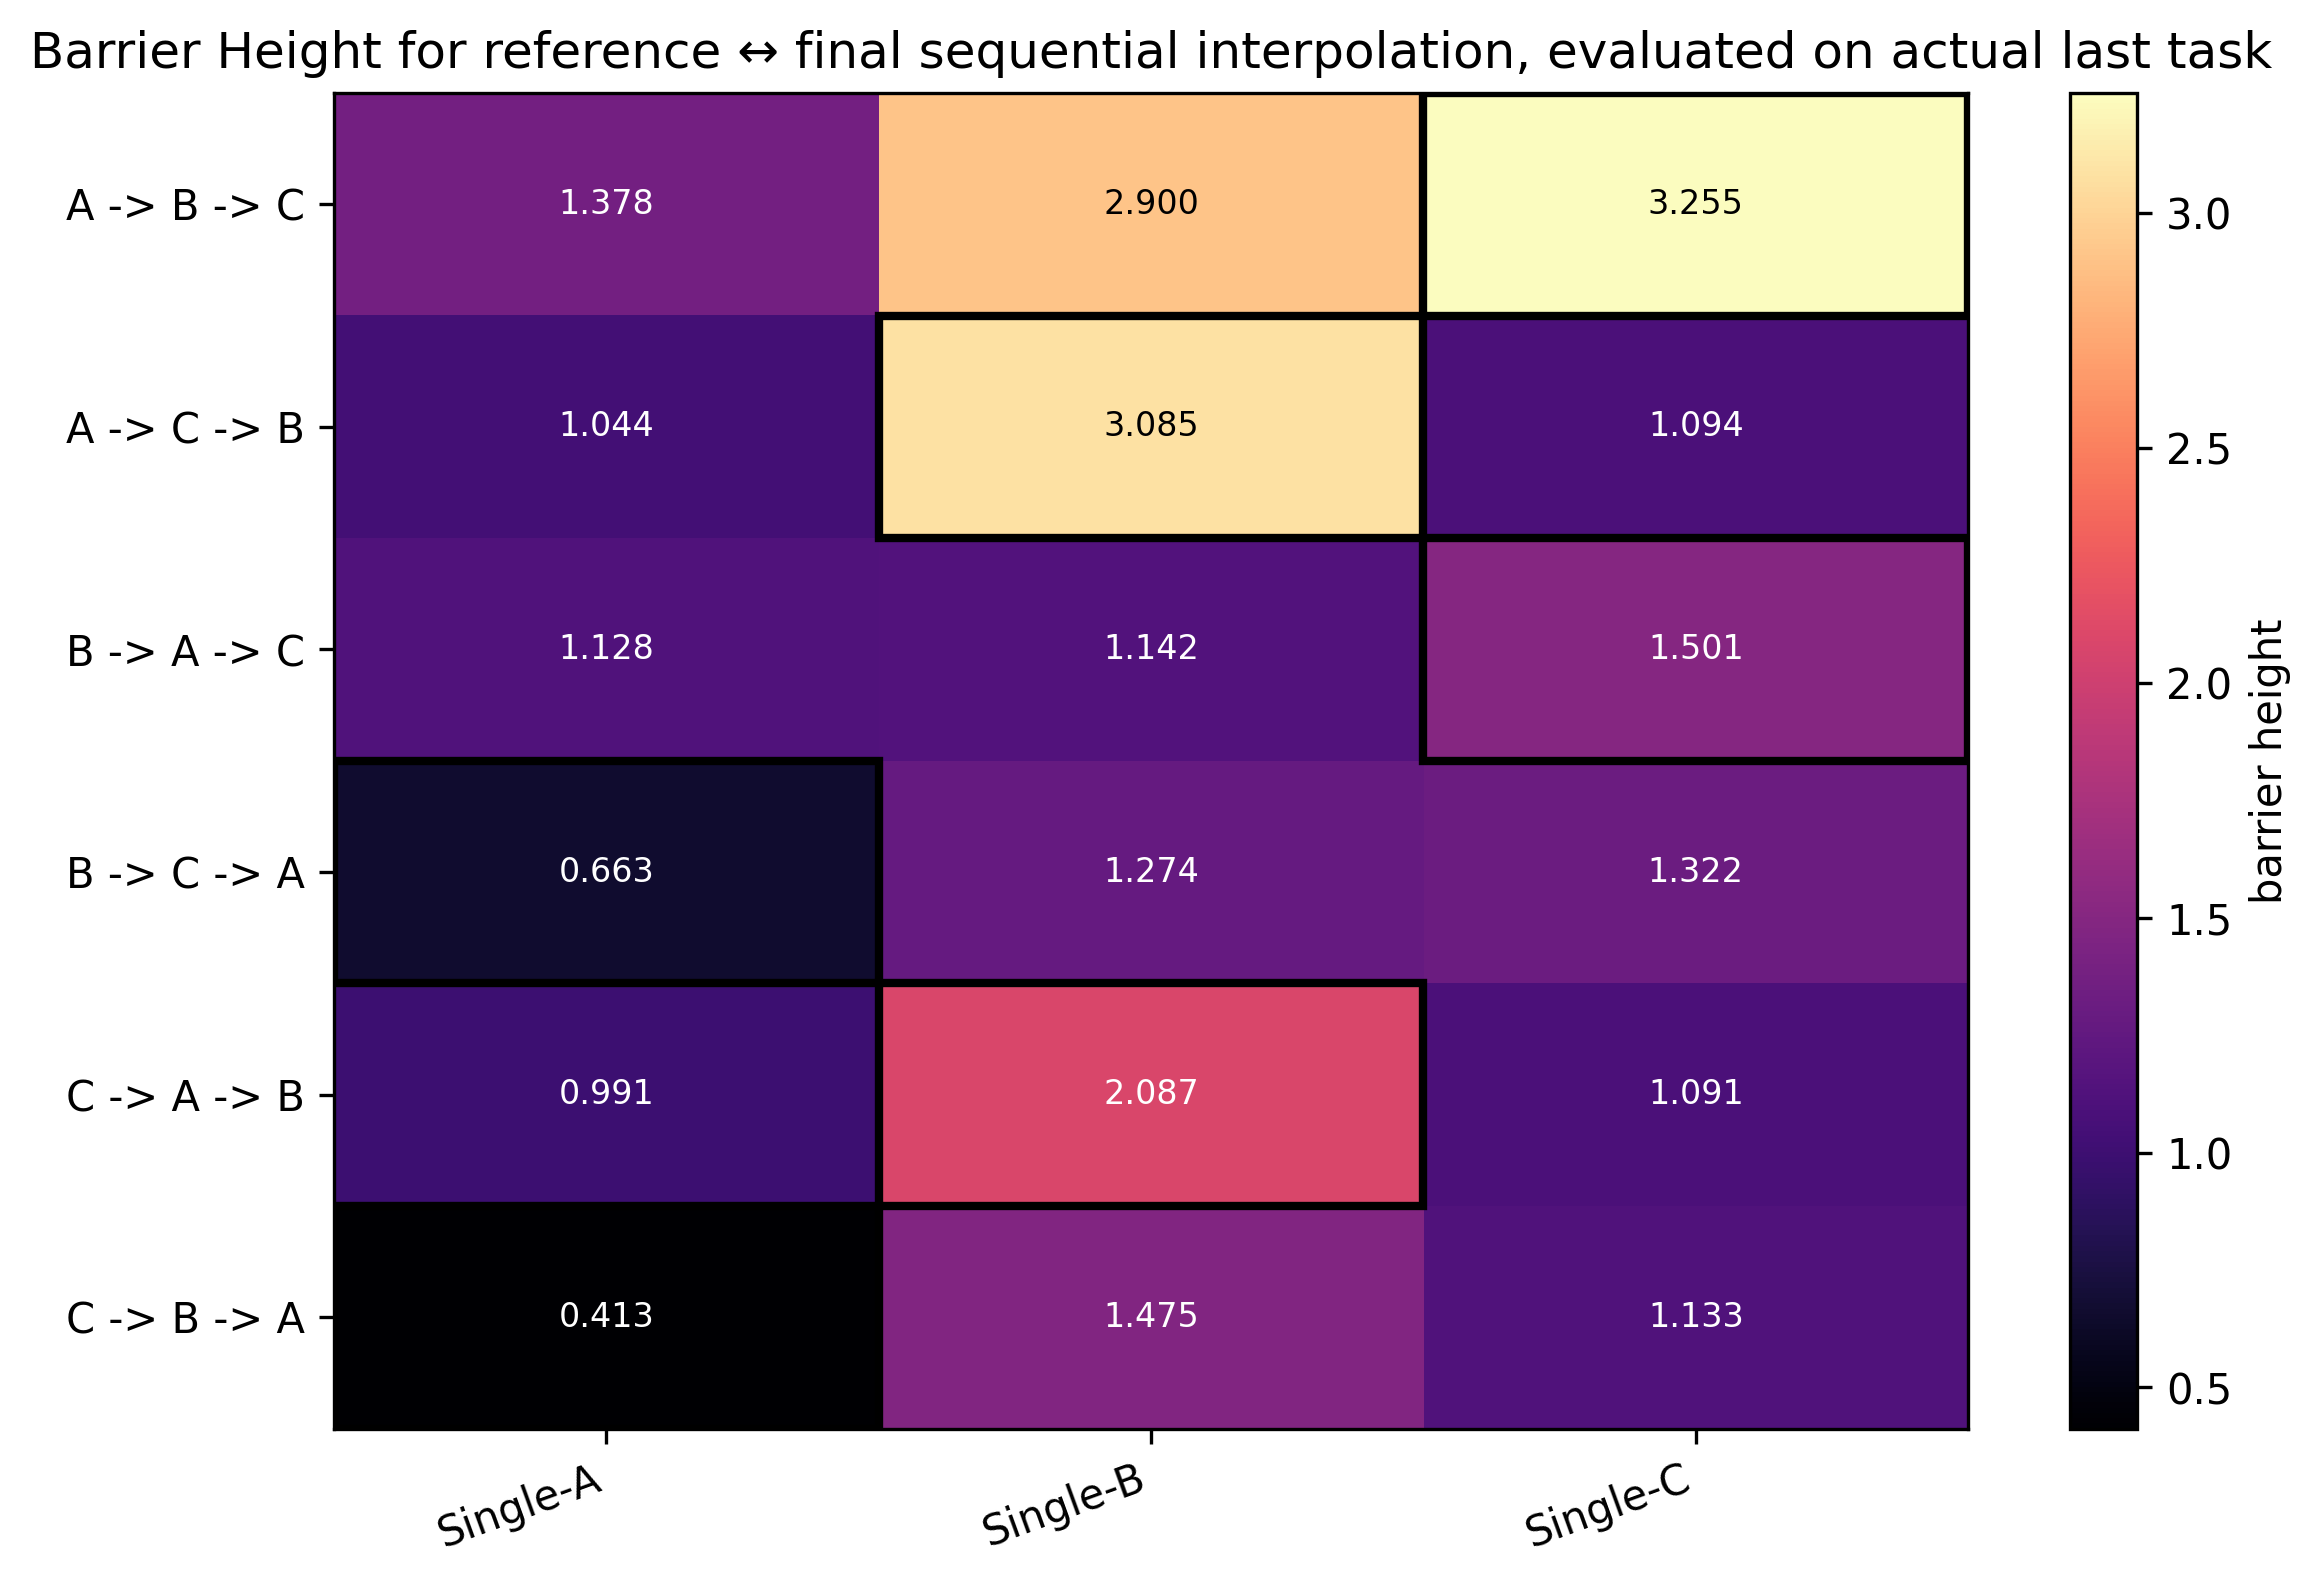
\includegraphics[width=\linewidth]{loss_barrier_height.png}
  \caption{Loss-barrier height on the actual last task.}
\end{subfigure}\hfill
\begin{subfigure}[t]{0.48\linewidth}
  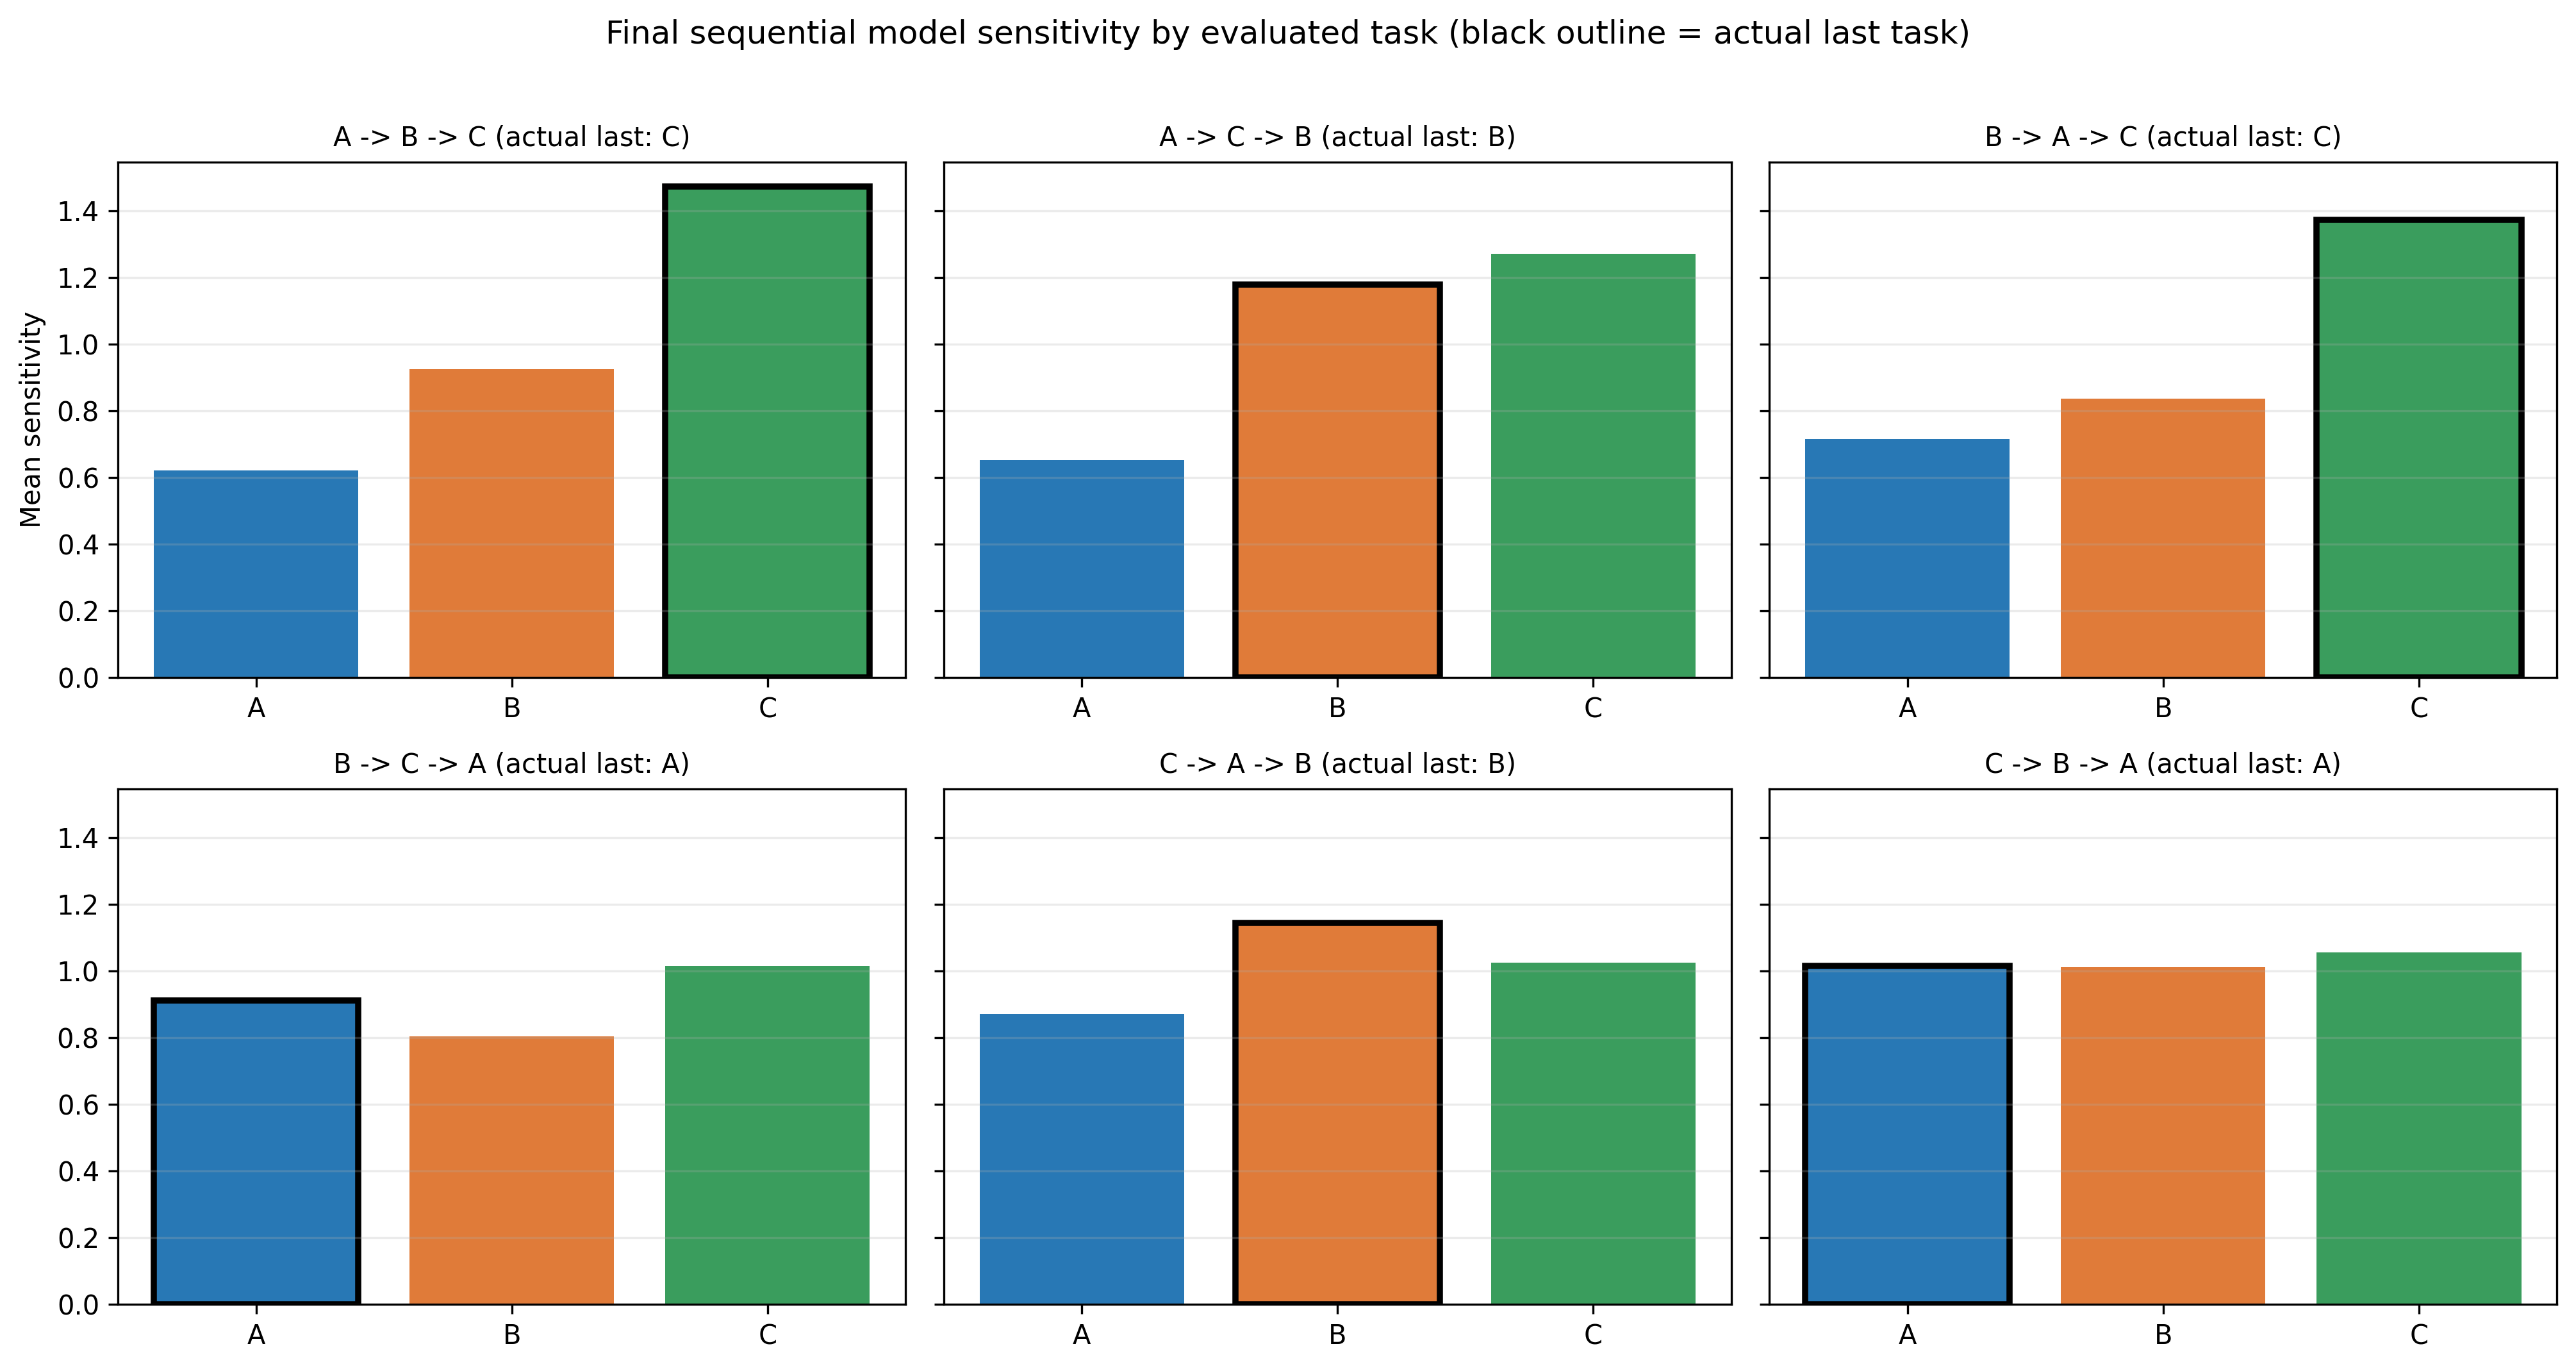
\includegraphics[width=\linewidth]{jacobian_sensitivity_by_order.png}
  \caption{Mean Jacobian sensitivity per task.}
\end{subfigure}
\caption{Supporting diagnostics. In both panels the black outline marks the actual last task (or its reference).}
\label{fig:diag}
\end{figure}

\section{Discussion}\label{sec:discussion}

The main finding is that the final checkpoint does contain information about the last task, but only when we look at what the network computes and not at where its weights are. CKA and feature drift compare representations on the same images, and they selected the last task reliably. Distances between the parameters instead selected the first task in every order. We did not test why, but a plausible explanation is that the first stage of sequential training is essentially the training of the corresponding single-task reference, starting from the same initialisation. The model would then begin close to that reference, and the later stages move it away from the references of the other two tasks by similar amounts. Under this reading, parameter distance mostly reflects the starting point of the history and not its end. This should be checked, for example by measuring the distance of the intermediate checkpoints to the references.

The shared initialisation also plays a role in how we read the weight-space results. Mirzadeh et al.\ \cite{mirzadeh2020} report linear connectivity between continual and multitask solutions when the initialisation is shared. In our case weight matching found nothing to align, which is what one expects when all models start from the same $\theta_0$. The weight-space result may therefore not carry over to models with different initialisations, which we did not test.

The Fisher result is harder to interpret. The direction that worked, ``low is recent'', would mean that the most recently learned task sits in a flatter region for its own data. That is an interesting statement, but with four correct out of six, two of them with small margins, and a full-order accuracy near chance, we cannot claim it as a reliable fingerprint. Its advantage is that it needs no reference models. Whether it holds up with more orders or seeds is an open question.

The forgetting results fit the general expectation: earlier tasks are damaged by later training even though their heads are frozen. Since the first task is forgotten more than the second in every order, it is natural to ask whether forgetting could also serve as a signal for the order, but we did not evaluate it as a predictor. Our forgetting is measured at the output through frozen heads, so the loss of accuracy reflects a change in the shared features. This fits the view of Hess et al.\ \cite{hess2024} that continually learned representations do forget, although we did not separate feature forgetting from output forgetting as they do, and we did not look at how well the representation supports new tasks (knowledge accumulation).

\paragraph{Limitations.} The study has several limits that matter for how far the conclusions go.
\begin{itemize}
  \item All results come from a single training run with seed 42. We have no estimate of the variance between runs.
  \item There are only six orders. One flipped prediction changes an accuracy by 16.7 points, and the orders share the same references.
  \item We use three small tasks with five classes each and one architecture. Other task sets, more tasks, or larger models may behave differently.
  \item Training lasted 20 epochs per task. Forgetting and the fingerprints might change with longer or shorter training.
  \item All checkpoints share one initialisation. This is why weight matching returned identity permutations, so we could not test whether it helps when models start from different initialisations.
  \item The first-task rule for weight distance was found after seeing the results.
  \item Loss-barrier and Jacobian results are diagnostics only, and the loss-barrier curves contain values we have not explained.
\end{itemize}

\section{Conclusion}\label{sec:conclusion}

We trained a ResNet18 on three CIFAR-100 tasks in all six orders and checked whether the final model reveals the task learned last. For RQ1, linear CKA identified the last task in 6 of 6 orders and feature drift in 5 of 6, both clearly above the 33\% baseline. The Fisher trace reached 4 of 6 when low values are read as recent, which we cannot separate from chance with six orders. L2 distance and cosine similarity of the weights got 0 of 6, also after weight matching, so the failure is not caused by permutation symmetry. For RQ2, weight distance reliably points to the first task, and together with CKA this recovers all six complete orders of three tasks. This does not extend to longer sequences, since the middle tasks remain undetermined. For RQ3, earlier tasks lose a large part of their accuracy after later training, while the last task by definition does not, and this was measured after 20 epochs only.

The natural next steps are to repeat the experiment with several seeds, to test longer training and more than three tasks, to examine the intermediate checkpoints to understand the first-task effect in weight space, to repeat weight matching with independently initialised models, where it is expected to matter, and to measure forgetting at the representation level in the sense of Hess et al.\ \cite{hess2024} to see whether it relates to the last-task signal in CKA.

\begin{thebibliography}{9}\small

\bibitem{ainsworth2023}
S.~K. Ainsworth, J.~Hayase and S.~Srinivasa.
\newblock Git Re-Basin: Merging models modulo permutation symmetries.
\newblock In \emph{International Conference on Learning Representations (ICLR)}, 2023.

\bibitem{he2016}
K.~He, X.~Zhang, S.~Ren and J.~Sun.
\newblock Deep residual learning for image recognition.
\newblock In \emph{IEEE Conference on Computer Vision and Pattern Recognition (CVPR)}, 2016.

\bibitem{hess2024}
T.~Hess, E.~Verwimp, G.~M. van~de Ven and T.~Tuytelaars.
\newblock Knowledge accumulation in continually learned representations and the issue of feature forgetting.
\newblock \emph{Transactions on Machine Learning Research}, 2024. arXiv:2304.00933.

\bibitem{kornblith2019}
S.~Kornblith, M.~Norouzi, H.~Lee and G.~Hinton.
\newblock Similarity of neural network representations revisited.
\newblock In \emph{International Conference on Machine Learning (ICML)}, 2019.

\bibitem{krizhevsky2009}
A.~Krizhevsky.
\newblock Learning multiple layers of features from tiny images.
\newblock Technical report, University of Toronto, 2009.

\bibitem{mccloskey1989}
M.~McCloskey and N.~J. Cohen.
\newblock Catastrophic interference in connectionist networks: The sequential learning problem.
\newblock \emph{Psychology of Learning and Motivation}, 24:109--165, 1989.

\bibitem{mirzadeh2020}
S.~I. Mirzadeh, M.~Farajtabar, D.~Gorur, R.~Pascanu and H.~Ghasemzadeh.
\newblock Linear mode connectivity in multitask and continual learning.
\newblock arXiv preprint arXiv:2010.04495, 2020.

\end{thebibliography}

\end{document}
